\documentclass[12pt,phd,times]{pkmthesis}
\usepackage{amsmath,graphicx,setspace,url,float}
\usepackage{pifont}
\usepackage{lscape,multicol,multirow,longtable,subfigure}
\usepackage{cite, bm}                           % Due to this hyberref will not work for references (PKM on 07/07/08)
\usepackage[english]{babel}
\usepackage[small,bf]{caption}    
\usepackage{tikz}
% Added on 26/08/08
%\usepackage{slashbox} 
\usepackage{csquotes}  
\usepackage{threeparttable}
%\usepackage{adjustbox}                    % Added on 24/10/08 (Senthil)
\setlength{\textfloatsep}{1cm}              % Spacing b/w  float and text (PKM 01/11/08)
%..........................................................................................................................................
\normalem                                   % Added on 01/07/08 to avoid underline in the references
\setlength{\abovecaptionskip}{8pt}          % Added on 08/07/08
\setlength{\belowcaptionskip}{8pt}          % Added on 08/07/08
%..........................................................................................................................................
\usepackage{hyperref}
\usepackage{extra_functions}
%\input{pagesetup_pkm_twoside.tex}           % Modified on 06/07/08, 10/07/08, 15/07/08
%\input{pagesetup_pkm_singleside.tex}       % For Single Sided Document 
\input{pagesetup_pkm_middleside.tex}       % Middle alignment 
\raggedbottom                               % o6/08/08  (Remove Unnecessary space b/w paragraphs)
%******************************************************************************************************************************************

\begin {document}
\setcounter{page}{1} \pagenumbering{roman}  % 03/07/08
\doublespacing                              % or use \baselineskip 12pt (12, 18 and 24)
%*************************************************** FRONT PAGES**********************************************
%\thispagestyle{empty}
%\pdfbookmark{Title}{Title}
%\begin{center}
\LARGE
{\textbf{Lightweight Blockchain-Based Data Trading \\Scheme in Internet of Vehicles}}

\vspace*{0.13in}
{\large{\emph{A\\
report submitted in fulfillment for}}} \\
{\large{\textbf{\emph{Colloquium Project}}}} \\
\large{in} \\
\large{Computer Science and Engineering} \\
\large{By} \\
\large{\textbf{Tiyyagura Jeevan Reddy : 2023 BCS 069}} \\
\large{Under the Supervision of} \\
\large{\textbf{Dr. Amrendra Singh Yadav}} \\
\large{Department of Computer Science}
\end{center}

\begin{center}

\includegraphics[width=3cm]{FrontPages/ABV_IIITM_Logo.jpeg}
\end{center}

\centerline{\large{ABV-INDIAN INSTITUTE OF INFORMATION TECHNOLOGY}}
\centerline{\large{AND MANAGEMENT GWALIOR}}
\vspace*{0.05in}
\centerline{\large{GWALIOR, INDIA}}
\vspace*{0.05in}
\centerline{\large{JULY, 2026}}

%\thispagestyle{empty}
%\clearpage

\thispagestyle{empty}
\pdfbookmark{Title}{Title}
\begin{center}
\LARGE
{\textbf{Lightweight Blockchain-Based Data Trading \\Scheme in Internet of Vehicles}}

\vspace*{0.13in}
{\large{\emph{A\\
report submitted in fulfillment for}}} \\
{\large{\textbf{\emph{Colloquium Project}}}} \\
\large{in} \\
\large{Computer Science and Engineering} \\
\large{By} \\
\large{\textbf{Tiyyagura Jeevan Reddy : 2023 BCS 069}} \\
\large{Under the Supervision of} \\
\large{\textbf{Dr. Amrendra Singh Yadav}} \\
\large{Department of Computer Science}
\end{center}

\begin{center}

\includegraphics[width=3cm]{FrontPages/ABV_IIITM_Logo.jpeg}
\end{center}

\centerline{\large{ABV-INDIAN INSTITUTE OF INFORMATION TECHNOLOGY}}
\centerline{\large{AND MANAGEMENT GWALIOR}}
\vspace*{0.05in}
\centerline{\large{GWALIOR, INDIA}}
\vspace*{0.05in}
\centerline{\large{JULY, 2026}}

\thispagestyle{empty}

\clearpage
\thispagestyle{empty}
\pdfbookmark{Dedication}{Dedication}
%\include{FrontPages/Dedication}
%\mbox{}
%\thispagestyle{empty}
%\newpage
%\thispagestyle{empty}

%\clearpage
%\thispagestyle{empty}
\pdfbookmark{Certificate}{Certificate}

\begin{center}
{\Large \bf DECLARATION}
\end{center}

\vspace{0.5cm}

\noindent
I hereby certify that the work, which is being presented in the report/thesis, entitled ``Lightweight Blockchain-Based Data Trading Scheme in Internet of Vehicles'', in fulfillment of the requirements for the Colloquium Project and submitted to the institution, is an authentic record of my own work carried out during the period May 2026 to July 2026 under the supervision of Dr. Amrendra Singh Yadav. I have also cited the references for the text(s), figure(s), and table(s) wherever applicable.

\vspace{1cm}

\begin{center}
	\begin{tabular}{@{}p{0.48\textwidth}p{0.48\textwidth}@{}}
		Dated:  & {\bf{Signature of the candidate}}  
	\end{tabular}
\end{center}

\vspace{1.5cm}

\noindent
This is to certify that the above statement made by the candidate is correct to the best of my knowledge.

\vspace{1.5cm}

\begin{center}
	\begin{tabular}{@{}p{0.48\textwidth}p{0.48\textwidth}@{}}
		Dated: & {\bf{Signature of supervisor}} 
	\end{tabular}
\end{center}


%\mbox{}
%\thispagestyle{empty}
%\newpage
%\thispagestyle{empty}
%\clearpage

\thispagestyle{empty}
\pdfbookmark{Acknowledgement}{Acknowledgement}
%\begin{acknowledgments}
\begin{center}
{\LARGE \bf Acknowledgements}
\end{center}
\noindent I express my sincere gratitude to my supervisor, Dr. Amrendra Singh Yadav, for his guidance, insightful feedback, and constant encouragement throughout this Colloquium Project (May 2026 to July 2026). His advice provided clear direction while giving me the independence to design and implement the Lightweight Blockchain-Based Data Trading (LBDT) framework.

Working on this project has deepened my understanding of decentralized security, game-theoretic auctions, and machine learning applications in the Internet of Vehicles (IoV). I am grateful to the Department of Computer Science and ABV-IIITM Gwalior for providing the necessary computational facilities, simulation platforms, and academic environment to carry out this work.

I would also like to thank the faculty members and fellow students whose technical discussions and constructive critiques helped refine the methodology and implementation of this report.

\vspace{1cm}
\begin{flushright}
\textit{\textbf{Tiyyagura Jeevan Reddy}}\\
\textit{2023 BCS 069}
\end{flushright}



%\end{acknowledgments}

\thispagestyle{empty}
\clearpage

\thispagestyle{empty}
%\pdfbookmark{Abstract}{Abstract}
%\renewcommand{\baselinestretch}{1.1}
%\include{FrontPages/Abstract2}
{\renewcommand{\baselinestretch}{1.5}
{%\small\normalsize
\begin{center}
	{\bf{Abstract}}
\end{center}
{\em{\noindent The fast growth of the Internet of Vehicles (IoV) facilitates smart transportation applications, such as real time traffic monitoring, collision detection and cooperation sensing. However, achieving continuous data exchange between self-interested vehicles requires a suitable organization of data trading. Conventional data trading systems fail due to a number of disadvantages, such as single point of failure, privacy breach, high latency, as well as vulnerability to dishonest activity like free riding or data manipulation. 

In order to tackle these issues, this report proposes a solution called the Lightweight Blockchain-Based Data Trading (LBDT) scheme. LBDT is a decentralized approach that is specifically created for vehicular scenarios characterized by extensive mobility. The LBDT is based on a two-layer chained ledger with keyblocks responsible for the maintenance of epoch-related parameters, alongside global reputation history, and a second type of records named microblocks that are used to keep the track of the localized data transactions with a high frequency. To ensure a satisfactory degree of trust in transactions, the model is reliant on the so-called Aged Gompertz Reputation Model based on historical frequency plots, time-decay metrics, and machine-learning-based classifiers, i.e., the ($p_{honest}$) system that uses results from the operation with node interaction database. In addition to this, a mechanism that takes into account reputation concerning double auction is employed, which allows the transaction delays and reputation penalties that will influence the price of a seller.

In an attempt to keep the consensus latency and the complexity of messages low, LBDT implements an Elliptic Curve Verifiable Random Function (EC-VRF) for random committee leader selection and a Gosig BFT consensus protocol so that the complexity of local communication drops down to $5N-3$ messages per round of consensus. The use of the dynamic geographical zoning strategy splits and merges the sharded clusters according to the load and density of vehicles.Simulation experiments conducted across 1,000 vehicles and 400 Roadside Units (RSUs) using SUMO and Veins demonstrate an average transaction confirmation latency of 2.4828 seconds, an ML classifier ROC-AUC of 0.9991, and a maximum committee malicious reputation ratio of 19.4\%, significantly below the 33.3\% BFT safety bound.

\par\vspace{1em}
\textbf{Keywords:} Internet of Vehicles, Blockchain, Double Auction, Proof-of-Reputation, Machine Learning, Byzantine Fault Tolerance, Data Trading.

	}}}}	
\thispagestyle{empty}
\clearpage
%\mbox{}
%\thispagestyle{empty}
%\newpage
%..........................................................................................................................................
% For the fancy chapters (Don't remove these lines- 03/07/08)
\clearpage
\thispagestyle{empty}
\dominitoc
\dominilof
\dominilot
\fancyhf{} \fancyhead[LE]{\bfseries\small{\leftmark}}
\fancyhead[RO]{\bfseries\small{\rightmark}}
\fancyfoot[CE,CO]{\bfseries\thepage}
%..........................................................................................................................................
%TABLE OF CONTENTS
\renewcommand{\baselinestretch}{1}
\pdfbookmark[0]{Index}{index}
\pdfbookmark[1]{Contents}{toc}
\fancyhead[LE]{\bfseries\small{Contents}}
\fancyhead[RO]{\bfseries\small{Contents}}
\tableofcontents
\clearpage
%.........................................................................................................................................
 %LIST OF FIGURES
\pdfbookmark[1]{List of Figures}{lof}
\addstarredchapter{List of Figures}       % PKM 05/07/08 (For more options  refer minitoc.pdf on page 36)
\fancyhead[LE]{\bfseries\small{List of Figures}}
\fancyhead[RO]{\bfseries\small{List of Figures}}
\listoffigures
\clearpage
% %..........................................................................................................................................
% % LIST OF TABLES
\pdfbookmark[1]{List of Tables}{lot}
\addstarredchapter{List of Tables}         % or use \mtcaddchapter[List of Tables] [Please Refer minitoc.pdf]
\fancyhead[LE]{\bfseries\small{List of Tables}}
\fancyhead[RO]{\bfseries\small{List of Tables}}
\listoftables
\clearpage
% %..........................................................................................................................................
% LIST OF ACRONYMS
\fancyhead[LE]{\bfseries\small{List of Acronyms}}
\fancyhead[RO]{\bfseries\small{List of Acronyms}}
\pdfbookmark[1]{List of Acronyms}{loa}
\addstarredchapter{List of Acronyms}
\chapter*{List of Acronyms}

\begin{longtable}{ll}

% A
AUC & Area Under Curve \\

% B
BFT & Byzantine Fault Tolerance \\

% C
CP & Clearing Price \\

% D
DSRC & Dedicated Short-Range Communications \\

% E
ECDSA & Elliptic Curve Digital Signature Algorithm \\
EC-VRF & Elliptic Curve Verifiable Random Function \\

% I
IoV & Internet of Vehicles \\
IP & Internet Protocol \\

% L
LBDT & Lightweight Blockchain-Based Data Trading \\

% M
ML & Machine Learning \\

% O
OBU & On-Board Unit \\

% P
PoR & Proof-of-Reputation \\
PoW & Proof-of-Work \\

% R
ROC & Receiver Operating Characteristic \\
RSU & Roadside Unit \\

% S
SECP & Standards for Efficient Cryptography Protocol \\
SUMO & Simulation of Urban MObility \\

% T
TCP & Transmission Control Protocol \\
TPS & Transactions Per Second \\
TraCI & Traffic Control Interface \\

% V
VANET & Vehicular Ad-Hoc Network \\
VRF & Verifiable Random Function \\

\end{longtable}

\clearpage
%..........................................................................................................................................
% LIST OF SYMBOLS
\fancyhead[LE]{\bfseries\small{List of Symbols}}
\fancyhead[RO]{\bfseries\small{List of Symbols}}
\pdfbookmark[1]{List of Symbols}{los}
\addstarredchapter{List of Symbols}
%\include{FrontPages/Symbols}
\clearpage
%..........................................................................................................................................
\fancyhf{}
\fancyhead[LE]{\bfseries\small{\leftmark}}
\fancyhead[RO]{\bfseries\small{\rightmark}}
\fancyfoot[CE,CO]{\bfseries\thepage}
\setcounter{page}{1} \pagenumbering{arabic}
\renewcommand{\labelenumi}{(\roman{enumi})}   % Added on 09/08/2008
%*******************************************************************************************************************************************************************************************


%************************************************ BEGIN CHAPTERS **********************************************
%\fancychapter{Introduction}
\chapter{Introduction}
\vspace{-1cm}

\noindent \rule{\textwidth}{0.01in}
\emph{This chapter lays the foundation for this research by providing an overview of the Internet of Vehicles (IoV) and the critical challenges associated with decentralized data trading among vehicular nodes. Furthermore, it outlines the key motivations, problem statement, project objectives, major contributions, and structural organization of this report.}
\section{Background and Overview}\label{sec:intro_background}
\noindent In recent years, the rapid growth of autonomous driving and connected vehicular networks has accelerated the development of the Internet of Vehicles (IoV).IoV makes it possible for different vehicles to communicate with one another and also with road infrastructures making it as a framework for cooperative intelligent transportation system (C-ITS) \cite{chen2025lbdt}. Applications such as automated collision avoidance, real-time dynamic rerouting (for example, through vehicle-to-vehicle (V2V) communication), cooperative environmental sensing and road hazard detection are based on the constant sharing of sensor and telemetry data \cite{javaid2020scalable}.

However, data sharing in vehicular networks cannot be based only on goodwill. Data gathering uses local computational and storage resources as well as energy in the on-board units (OBUs). That is why cars in vehicular networks act in a self-interested way and need incentives for sharing data \cite{kang2019toward}. Data trading protocols enable data-buyers (e.g.. autonomous vehicles needing real-time road condition updates) to buy verified data from data-sellers (e.g., cars/vehiceles equipped with LiDAR or camera arrays).

Conventional vehicle data markets depend on centralized hardware that connects sellers, buyers, and allows transactions. While it is easy to implement, having a centralized server raises the possibility of failure, increases communication delays across hops in wireless networks, exposes the whereabouts of cars, and creates chances of platform manipulation \cite{michelin2018speedychain}. Existing literature advocates for decentralized trading based on blockchain technology as a new solution that offers reliable and transparent waiting for payments without the use of any centralized parties \cite{liu2018computation, firdaus2021blockchain}.

\section{Motivation and Key Challenges}\label{sec:intro_motivation}
\noindent Deploying standard blockchain technologies directly in high-mobility IoV environments introduces several severe technical bottlenecks:

\begin{enumerate}
    \item \textbf{Transaction Confirmation Latency vs. Mobility Dynamics:} Standard Proof-of-Work (PoW) or traditional Proof-of-Stake (PoS) blockchains suffer from low transaction throughput (TPS) and multi-minute confirmation delays \cite{nakamoto2008bitcoin}. In vehicular networks, where topologies change rapidly within seconds, transaction latencies exceeding a few seconds cause market mismatches and outdated data delivery.
    \item \textbf{Dishonest Behaviors and Identity Spoofing:} Malicious or opportunistic vehicular nodes may transmit fabricated, noisy, or incomplete data to maximize profits. Without an adaptive trust evaluation model, bad actors can exploit trading protocols through selective packet dropping, free-riding, or collusion attacks \cite{rosenstatter2018modelling}.
    \item \textbf{Market Inefficiency and Unfair Pricing:} Traditional auction protocols often fail to account for data freshness (latency) and seller reputation simultaneously. Unregulated pricing can discourage honest participants while rewarding dishonest sellers who offer low-quality data at predatory prices \cite{guan2020towards}.
    \item \textbf{High Consensus Communication Overhead:} Classical Byzantine Fault Tolerance (BFT) consensus protocols require $O(N^2)$ message complexity during commit rounds \cite{lamport1982byzantine}. In dense urban intersections with hundreds of participating Roadside Units (RSUs), this communication burden saturates the wireless channel and causes severe network congestion.
\end{enumerate}

\section{Problem Statement}\label{sec:intro_problem}
\noindent With the dynamic nature of the vehicular network that features time-dependent topology, changing vehicle density, and maybe compromised nodes, this project will focus on the creation, achievement, and assessment of the lightweight blockchain-based data trading method (LBDT). Specifically, the method must ensure a low confirmation time, high transaction capacity, solid protection against malicious actions, just market value, and scalable consensus under strict vehicle mobility limitations.

\section{Project Objectives}\label{sec:intro_objectives}
\noindent In order to address the issues described above this project has the following specific technical goals:
\begin{enumerate}
    \item \textbf{Dual Parallel Chain Architecture:} Create a separate architecture for Keyblocks (keeping epoch setups and the global reputation list) and Microblocks (sensing localized high productivity data trades).
    \item \textbf{Aged Gompertz Reputation \& ML Classifier:} Create a realtime model which is based on the transaction frequency, aging effects, and a ML-based Logistic Regression classifier ($p_{honest}$) to estimate and weed out bad performing nodes.
    \item \textbf{Reputation-Aware Double Auction:} Create a double auction protocol that would adjust the selling price of sellers based on the execution time and node reputation in order to provide honest market clearing prices.
    \item \textbf{Lightweight EC-VRF \& Gosig BFT Consensus:} Use Elliptic Curve Verifiable Random Function (EC-VRF) for unpredictable committee leader selection plus high performance Gosig BFT consensus protocol which limits the communication overhead to ($5N-3$) messages.
    \item \textbf{Dynamic Zone Sharding:} Use dynamic geographic zone rules based on utility load scores ($U_z$) to shift overutilized clusters and merge underutilized zones.
    \item \textbf{Co-Simulation Framework:} Ensure the functionality of the developed frame-
    work by combining the Python logic with C++ OMNeT++/Veins simulation and simulation program SUMO.
\end{enumerate}

\section{Major Technical Contributions}\label{sec:intro_contributions}
\noindent This report summarizes the major technical contributions of the project, including the following developments:
\begin{itemize}
    \item An Aged Gompertz Reputation Model which has been developed that has enabled log transformed interaction counts and an adjustable parameter adjustment method with the Logistic Regression classifier achieving the empirical ROC-AUC of 0.9991 for 10,400 dataset samples.
    \item A Double Auction matching algorithm that has been developed including a penalty function for bid losses such as  $loss = \alpha_1 (\Delta t)^{\beta_1} + \alpha_2 (1 - Rep_i)^{\beta_2}$, ensuring that sellers characterized by low reputation or by high latency are penalized appropriately.
    \item A consensus pipeline has been created that includes the SECP256k1 EC-VRF leader election as well as the four-phase Gosig BFT consensus engine limiting the use of messages to ($5N – 3$) per step of consensus.
    \item A thorough co-simulation pipeline has been created that allows for SUMO, Veins, OMNeT++, and Python to be implemented, which demonstrates an average transaction confirmation time of 2.4828 seconds and limit on the malicious reputation levels of the committee below 19.4\% (well below the permissible level of 33.3\% with respect to BFT).




\end{itemize}

\section{Organization of the Report}\label{sec:intro_organization}

\noindent The remainder of this report is organized as follows:

{\emergencystretch=2em
\begin{itemize}
    \item \textbf{Chapter 2 (Literature Review):} Reviews prior art in vehicular networks, blockchain-based data trading, reputation systems, double auctions, and BFT consensus.

    \item \textbf{Chapter 3 (Problem Statement \& System Model):} Formulates the formal mathematical model, system components, and security threat model.

    \item \textbf{Chapter 4 (Implemented LBDT Scheme \& Methodology):} Presents the technical design and mathematical formulation of the dual parallel chain, reputation model, ML classifier, double auction engine, EC-VRF Gosig BFT, and dynamic sharding logic.

    \item \textbf{Chapter 5 (Experiment and Results):} Details the experimental setup, simulation environment, empirical performance metrics, and comparative evaluation graphs.

    \item \textbf{Chapter 6 (Conclusions and Future Scope):} Concludes the report with a summary of findings, limitations, and future research directions.
\end{itemize}
}\label{chap:intro}
%\clearpage
%\mbox{}
%\thispagestyle{empty}
%\newpage
%\fancychapter{Literature Review}
\chapter{Literature Review}
\vspace{-1cm}
\noindent \rule{\textwidth}{0.01in}
\emph{In secure vehicular data trading, prior studies have investigated different paradigms. This chapter discusses the previous research done in five major domains: VANETs, blockchain technology in IoV, reputation-based trust management, double auction mechanism, and Byzantine Fault Tolerant consensus algorithms.}
\section{Overview of Vehicular Data Trading Schemes}\label{sec:lit_data_trading}

{\emergencystretch=2em
\noindent
Recently, vehicular data trading has become a key paradigm for implementing cooperative autonomous driving and smart transportation systems \cite{chen2025lbdt}. The advanced sensors like LiDAR, radar, and high-resolution cameras can produce tremendous amounts of data on local environmental conditions \cite{kang2019toward}. Traditional data trading methods depend on centralized cloud services for data management and pricing. However, centralized systems bring various problems with them, like the possibility of single point of failure, provider lock-in effect, added latency in multihop systems, and extensive chances of tracking user mobility. Decentralized systems (P2P) quickly gained popularity as a scalable option.
}

\section{Blockchain Applications in Vehicular Networks}\label{sec:lit_blockchain}

\noindent
Blockchain technology has provided the means of achieving decentralized and immutable transaction recording and smart contract executing \cite{nakamoto2008bitcoin}. In case of vehicular ad-hoc networks (VANETs), consortium blockchains have been used for ensuring authentication, data sharing, and resource allocation without the use of trusted or centralized authorities \cite{yang2019privacy, firdaus2021blockchain}. For instance, Javaid et al. \cite{javaid2020scalable} proposed a trust management framework based on consortium blockchain for IoV data validation. Michelin et al\cite{michelin2018speedychain}. discussed SpeedyChain, which separates raw payload from blockchain ledger in order to enhance transaction efficiency in smart cities. 
{\emergencystretch=2em
\noindent
Nevertheless, monolithic blockchains do not work in networks with a high density of vehicles because of rapid size of storage, slow propagation of blocks and transaction concluding latencies \cite{liu2018computation}. Dual-chain architecture aimed at making microtransactions site independent from macro-state consensus thus looks very promising \cite{chen2025lbdt}.
}

\section{Reputation Systems and Trust Management}\label{sec:lit_reputation}

\noindent
In the case of vehicular communication, the open nature of the wireless medium facilitates
the transmission of erroneous or fabricated information by malicious or compromised
nodes, affecting the efficiency of functioning of the market\cite{rosenstatter2018modelling}. Traditional models of trust rely on static feedback score or average values, which do not allow them to adapt to the dynamic nature of behavior of nodes, strategies of collusion, and the processes ofwhitewashing \cite{cui2019extensible}. 

Gompertz function has proven to be a good instrument for modeling non-linear and sigmoidal behavior in biological and trust growth processes. By introducing the concept of interaction recency, it becomes possible to make dishonest nodes pay for their malfeasance immediately \cite{chen2025lbdt}. Moreover, the introduction of machine learning classification models, for instance, Logistic Regression or Support Vector Machines allows detecting the instances of non-honest behavior even before they are committed \cite{scikit-learn}.

\section{Double Auction Market Mechanisms}\label{sec:lit_auction}

\noindent
In auction theory a systematic approach is taken to match numerous data sellers with a number of data buyers in cases of dynamic supply and demand conditions \cite{guan2020towards}. when conventional one-sided auctions or fixed prices cannot perform the function of clearing the market when sellers are competing at the same time. 

Double auctions make it possible for buyers to place their bidding price ($BP$) and sellers to place their asking price ($SP$). However, in standard double auctions the assumption is that all data sellers provide data of the same quality and transmission time. In the case of vehicular networks, it becomes much more difficult, as the value of the data falls rapidly in time and the mechanism of the market must include such factors as the reputation penalty and transmission time delay in its calculation of the price for asking \cite{chen2025lbdt}.

\section{Consensus Protocols and Communication Overhead}\label{sec:lit_consensus}

\noindent
Consensus protocols prescribe the method by which decentralized nodes authenticate transactions and finalize block order. Practical Byzantine Fault Tolerance (PBFT) and its variations eliminate the need for energy-intensive PoW (Proof of Work) \cite{lamport1982byzantine}. Nevertheless, standard PBFT has a number of drawbacks, such as $O(N^2)$ message complexity that results in network overload in cases of high vehicular density.
To tackle this issue, a new process has been invented that introduces the usage of a verifiable Random Function (VRF) to randomly select small unpredictable groups of conference participants \cite{xie2023bephap}. If it is utilized along with multi-phase consensus systems like Gosig BFT, the communication difficulties are reduced to $O(N)$ (i.e.,$5N-3$ messages per round)level, allowing confirming the transactions in under 3 seconds even in dense vehicular scenarios \cite{chen2025lbdt}.

\section{Research Gaps Identified}\label{sec:lit_gaps}

\noindent
According to the literature review, four primary research gaps are found in current IoV data trading schemes:
\begin{enumerate}
    \item \textbf{Decoupling Latency from Consensus Complexity:} currently adopted IoV blockchain systems do not achieve sub-3 second confirmation latencies.

    \item \textbf{Static vs. Adaptive Reputation Modeling:}  most of the reputation systems use static thresholds which cannot identify adaptive attack modes that involve shifts between normal and malicious transactions. 

    \item \textbf{Ignoring Latency \& Reputation in Auction Pricing:} current double auction pricing mechanism determines the price based only on monetary bids, without considering data degradation and seller trustworthiness.

    \item \textbf{Lack of Dynamic Sharding for Mobility:} the adoption of fixed geographical zones leads to local bottlenecks, while vehicle clusters move constantly throughout city intersections.
\end{enumerate}

\label{chap:L_survey}
%\clearpage
%\mbox{}
%\thispagestyle{empty}
%\newpage

\chapter{Problem Statement}
\vspace{-1cm}
\noindent \rule{\textwidth}{0.01in}
\emph{This chapter details the formal problem formulation, threat model (including malicious sellers/buyers, collusion, and BFT committee corruption), and overall system architecture governing the LBDT framework.}
\section{System Architecture and Modeling}\label{sec:problem_system_model}
\noindent The Lightweight Blockchain-Based Data Trading (LBDT) ecosystem operates within a multi-zone urban Internet of Vehicles (IoV) environment. The system models three primary entities:

\begin{enumerate}
    \item \textbf{Vehicles ($V = \{v_1, v_2, \dots, v_M\}$):} Mobile nodes equipped with On-Board Units (OBUs) and wireless communication interfaces (IEEE 802.11p DSRC / C-V2X). Vehicles act dynamically as \textbf{Data Buyers} (seeking real-time traffic updates, sensor feeds, or road hazard alerts) or \textbf{Data Sellers} (offering verified sensor payloads for financial rewards).
    \item \textbf{Roadside Units ($R = \{r_1, r_2, \dots, r_K\}$):} Fixed roadside infrastructure nodes located along intersections and highway segments. RSUs possess higher computational, storage, and networking capacities. RSUs act as \textbf{Zone Authority Nodes}, hosting consensus committees, executing double auctions, and maintaining local ledger states.
    \item \textbf{Geographic Zones ($Z = \{z_1, z_2, \dots, z_P\}$):} Dynamically sharded spatial partitions covering the urban road network. Each zone $z_p$ is managed by a subset of localized RSUs and participating vehicular consensus nodes.
\end{enumerate}

\section{Security Threat Model and Adversary Assumptions}\label{sec:problem_threat_model}
\noindent In an open and decentralized IoV environment, we consider a hostile network environment where up to $f < N/3$ consensus nodes (and arbitrary vehicular participants) may be compromised or malicious. We classify potential attack vectors as follows:

\begin{itemize}
    \item \textbf{Data Tampering and Fraudulent Sellers:} Malicious sellers transmit corrupted, outdated, or fabricated sensor payloads after winning auction bids to harvest profits without incurring data acquisition costs.
    \item \textbf{Dishonest Bidding and Free-Riding Buyers:} Malicious buyers submit artificial bid prices ($BP$) or attempt to reuse single data purchases across unauthorized third-party vehicles without payment.
    \item \textbf{Selective Packet Dropping and Sybil Attacks:} Adversarial nodes deliberately drop relay packets, suppress consensus messages, or spawn multiple pseudonymous identities to distort reputation scores.
    \item \textbf{BFT Committee Corruption and Leader Bias:} Colluding RSUs attempt to bias committee leader selection, delay transaction confirmation, or insert invalid blocks into the ledger.
\end{itemize}

\section{System Objectives and Optimization Goals}\label{sec:problem_objectives}
\noindent The LBDT scheme has developed five major optimization goals to respond to these security problems and operational constraints, namely:
\begin{enumerate}
    \item \textbf{Latency Optimization:} Ensure less than 3 seconds end-to-end transaction confirmation latency for high-frequency trading operations in conditions of high vehicle density.
    \item \textbf{Reputation Accuracy:} Track the past interactions between nodes and apply penalties for dishonest behavior as per old Gompertz decay principle supported by machine learning ($p_{honest}$) so that malicious nodes are eliminated before entering auction matching.
    \item \textbf{Economic Fairness and Truthfulness:} Ensure that the price of the double auction clearing ($p_{win}$) reflects data freshness and seller reliability by implementing bid loss penalties.
    \item \textbf{Consensus Efficiency and Safety:}Ensure linear communication overhead through BFT of (5N-3) messages per round together with committee safety guarantee (malicious reputation ratio less than $< 33.3\%$).
    \item \textbf{Dynamic Load Balancing:} Ensure optimal utilization of zones ($U_z$) by  sharding split and merge operations.
\end{enumerate}
\label{chap:problem_statement}
%\clearpage
%\mbox{}
%\thispagestyle{empty}
%\newpage



\chapter{Methodology}
\vspace{-1cm}

\noindent \rule{\textwidth}{0.01in}

{\emergencystretch=2em
\emph{This chapter provides a comprehensive technical breakdown of the proposed LBDT methodology, detailing the dual parallel chain ledger, the Aged Gompertz Reputation Model, the Logistic Regression honesty classifier, the reputation-aware double auction engine, EC-VRF leader selection, Gosig BFT consensus, dynamic zone sharding, and the C++/Python simulation integration.}
}

\section{System Overview of the LBDT Framework}\label{sec:method_overview}
\noindent The Lightweight Blockchain-Based Data Trading (LBDT) framework is designed to provide secure, low-latency, and incentivized vehicular data exchange in dynamic Internet of Vehicles (IoV) environments. LBDT integrates five core architectural modules: (1) a Dual Parallel Chain Ledger Structure, (2) an Aged Gompertz Reputation Model enhanced by a Machine Learning Honesty Classifier, (3) a Reputation-Aware Double Auction Engine with Bid Loss Penalties, (4) an EC-VRF Leader Election and Gosig BFT Consensus Engine, and (5) a Dynamic Geographic Zone Sharding mechanism.

Figure~\ref{fig:lbdt_flowdiagram} illustrates the complete end-to-end data trading and consensus workflow in LBDT.


\begin{figure}[h!]
\centering
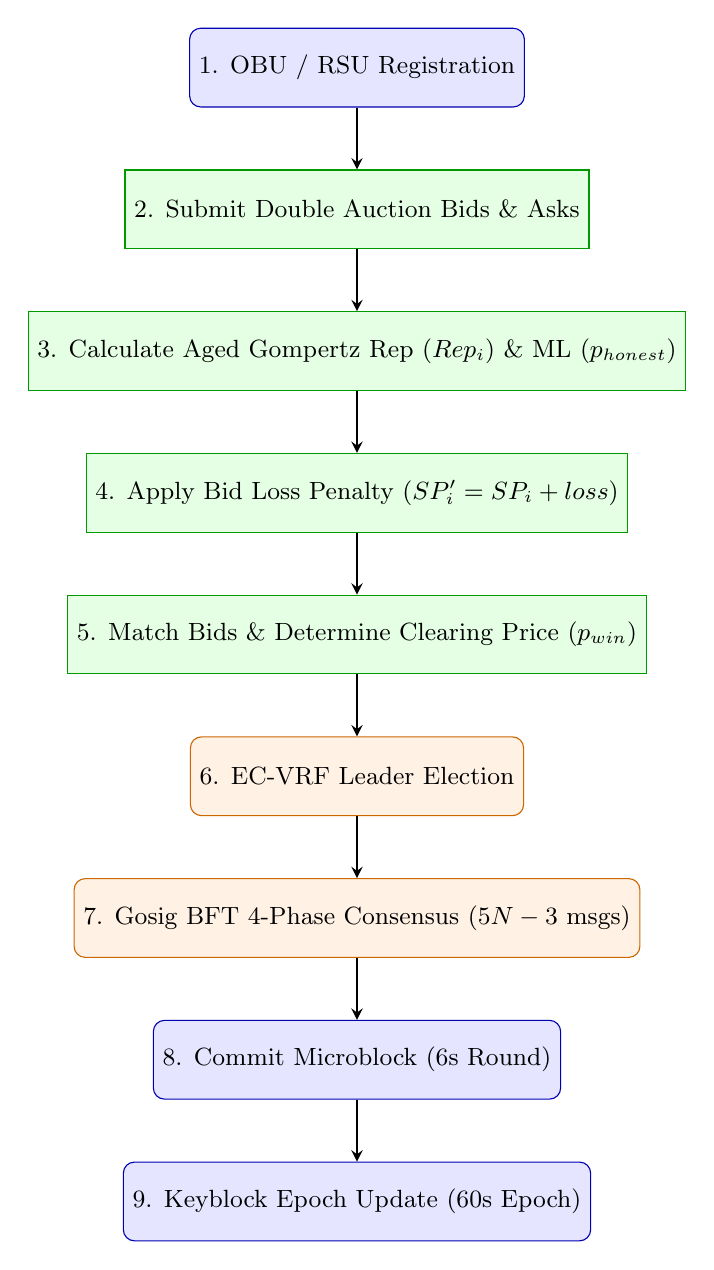
\begin{tikzpicture}[node distance=1.8cm and 2.5cm, auto]
% Styles
\tikzstyle{block} = [rectangle, draw=blue!70!black, fill=blue!10, rounded corners, minimum width=3.2cm, minimum height=1cm, text centered, font=\small]
\tikzstyle{process} = [rectangle, draw=green!60!black, fill=green!10, minimum width=3.2cm, minimum height=1cm, text centered, font=\small]
\tikzstyle{consensus} = [rectangle, draw=orange!80!black, fill=orange!10, rounded corners, minimum width=3.2cm, minimum height=1cm, text centered, font=\small]
\tikzstyle{arrow} = [thick,->,>=stealth]

% Nodes
\node (reg) [block] {1. OBU / RSU Registration};
\node (auc) [process, below of=reg] {2. Submit Double Auction Bids \& Asks};
\node (rep) [process, below of=auc] {3. Calculate Aged Gompertz Rep ($Rep_i$) \& ML ($p_{honest}$)};
\node (loss) [process, below of=rep] {4. Apply Bid Loss Penalty ($SP'_i = SP_i + loss$)};
\node (match) [process, below of=loss] {5. Match Bids \& Determine Clearing Price ($p_{win}$)};

\node (vrf) [consensus, below of=match] {6. EC-VRF Leader Election};
\node (bft) [consensus, below of=vrf] {7. Gosig BFT 4-Phase Consensus ($5N-3$ msgs)};
\node (micro) [block, below of=bft] {8. Commit Microblock (6s Round)};
\node (key) [block, below of=micro] {9. Keyblock Epoch Update (60s Epoch)};

% Arrows
\draw [arrow] (reg) -- (auc);
\draw [arrow] (auc) -- (rep);
\draw [arrow] (rep) -- (loss);
\draw [arrow] (loss) -- (match);
\draw [arrow] (match) -- (vrf);
\draw [arrow] (vrf) -- (bft);
\draw [arrow] (bft) -- (micro);
\draw [arrow] (micro) -- (key);

\end{tikzpicture}
\caption{End-to-End Workflow of the LBDT Data Trading and Consensus Protocol.}
\label{fig:lbdt_flowdiagram}
\end{figure}

\section{Dual Parallel Chain Ledger Architecture}\label{sec:method_dual_chain}
\noindent Traditional blockchain architectures struggle under high vehicular mobility due to the serial block creation bottleneck. LBDT resolves this by decoupling transactions into two distinct block structures:

\begin{enumerate}
    \item \textbf{Microblocks (Trading Chain):} High-frequency, localized blocks generated every short round interval ($\tau_{micro} = 6\text{ seconds}$). Microblocks pack data trading transactions, signed bids, matched clearing prices, and cryptographic data payload hashes. Microblocks require lightweight Gosig BFT validation to minimize latency.
    \item \textbf{Keyblocks (Macro Chain):} Epoch-level management blocks generated every macro epoch ($\tau_{key} = 60\text{ seconds}$). Keyblocks record global node reputation states, active RSU cluster topologies, zone sharding updates, and cryptographic proof anchor roots. Keyblocks use Proof-of-Work (PoW difficulty = 2) for macro-state finality.
\end{enumerate}

\section{Aged Gompertz Reputation \& Machine Learning Classifier}\label{sec:method_reputation}
\noindent To quantify node trustworthiness dynamically, LBDT introduces an Aged Gompertz Reputation Model. For any vehicular node $i$, the aged interaction score $r_n$ accumulates historical transaction feedback while decaying past interactions exponentially:

\begin{equation}
r_n = \left( \sum_{k=1}^{N_{trades}} \gamma^{n - 1 - k} \cdot \delta_k \right) \cdot \ln(N_{peers})
\end{equation}

\noindent where $\gamma = 0.95$ represents the aging decay factor, $\delta_k \in \{+1, -1\}$ denotes positive or negative transaction feedback, $n$ is the current transaction sequence index, and $N_{peers}$ is the total number of distinct trading partners.

The base reputation score $Rep_i$ is governed by a modified Gompertz sigmoidal growth function:

\begin{equation}
Rep_i = a_{adapt} \cdot \exp\left( - b_{adapt} \cdot \exp\left( - c \cdot r_n \right) \right)
\end{equation}

\noindent where $c = 0.1$ is the growth rate constant. To counteract adaptive malicious strategies (e.g., oscillating between honest and dishonest trades), LBDT incorporates a Logistic Regression ML classifier. The classifier evaluates a 4-dimensional telemetry feature vector $\mathbf{x}_i$:

\begin{equation}
\mathbf{x}_i = \left[ \text{honest\_trades}_i, \; \text{cheated\_trades}_i, \; \text{norm\_drop\_rate}_i, \; \text{bft\_responses}_i \right]^T
\end{equation}

The predicted honesty probability $p_{honest} = \sigma(\mathbf{w}^T \mathbf{x}_i + b)$ adaptively adjusts the Gompertz structural parameters:

\begin{align}
a_{adapt} &= a \cdot p_{honest} \qquad (a = 1.0) \\
b_{adapt} &= b + 3.0 \cdot (1 - p_{honest}) \qquad (b = 1.0)
\end{align}

If a node behaves maliciously, $p_{honest} \to 0$, causing $a_{adapt} \to 0$ and $b_{adapt} \to 4.0$, which instantly depresses $Rep_i$ to near zero.

\section{Reputation-Aware Double Auction Mechanism}\label{sec:method_auction}
\noindent Data trading within each zone is settled via a reputation-aware double auction. Data buyers submit bids $BP_j = (v_j, p_j^{\text{bid}})$, and data sellers submit asks $SP_i = (v_i, p_i^{\text{ask}}, \Delta t_i)$. To prevent low-reputation or high-latency sellers from exploiting the market, seller ask prices are adjusted by a bid loss penalty function:

\begin{equation}
loss_i = \alpha_1 \cdot (\Delta t_i)^{\beta_1} + \alpha_2 \cdot (1 - Rep_i)^{\beta_2}
\end{equation}

\noindent where $\alpha_1 = 0.5, \beta_1 = 1.2, \alpha_2 = 1.0, \beta_2 = 2.0$, and $\Delta t_i$ represents the sensor data generation delay. The adjusted seller price $SP'_i$ is formulated as:

\begin{equation}
SP'_i = SP_i + loss_i
\end{equation}

Buyers are sorted in descending order of $BP_j$, and sellers are sorted in ascending order of $SP'_i$. The matching engine identifies the maximum index $m$ satisfying $BP_m \ge SP'_m$. The unified transaction clearing price $p_{win}$ is calculated as:

\begin{equation}
p_{win} = \min\left( BP_m, \; SP'_{m+1} \right)
\end{equation}

\section{EC-VRF Leader Election and Gosig BFT Consensus}\label{sec:method_consensus}
\noindent To achieve lightweight consensus without $O(N^2)$ message overhead, LBDT executes consensus in two steps:

\begin{enumerate}
    \item \textbf{EC-VRF Leader Election:} Committee nodes generate a verifiable random hash $H_{vrf} = \text{VRF\_Hash}(SK_i, seed)$ over the SECP256k1 elliptic curve using $seed = \text{SHA256}(\text{last\_keyblock} \parallel \text{step} \parallel \text{zone\_id})$. The node with the minimum $H_{vrf}$ value is elected consensus leader.
    \item \textbf{Gosig BFT Protocol:} The leader broadcasts the candidate microblock. Consensus proceeds across 4 phases: \textit{Proposal}, \textit{Prepare}, \textit{Tentative Commit}, and \textit{Commit}. By leveraging aggregate multisignatures, total message complexity is strictly bounded to:
    \begin{equation}
    M_{bft} = 5N - 3
    \end{equation}
    where $N$ is the number of active committee RSUs.
\end{enumerate}

\section{Dynamic Geographic Zone Sharding}\label{sec:method_sharding}
\noindent To handle fluctuating vehicle densities across urban corridors, LBDT implements dynamic geographic sharding. Each zone $z_p$ continuously calculates a utility load score $U_z$:

\begin{equation}
U_z = 0.3 \left( \frac{V_z}{V_{max}} \right) + 0.3 \left( \frac{T_{wait}}{T_{limit}} \right) + 0.4 \cdot R_{adv}
\end{equation}

\noindent where $V_z$ is vehicle count, $T_{wait}$ is average transaction queueing delay, and $R_{adv}$ represents adversarial node ratio. When $U_z > 0.85$, the zone automatically splits into sub-zones. Conversely, when $U_z < 0.20$, adjacent sparse zones merge.

\section{C++ Veins to Python Simulation Architecture}\label{sec:method_integration}
\noindent The system implementation couples the C++ OMNeT++/Veins discrete-event network simulator (\texttt{LBDTApp.cc}) with a Python backend server (\texttt{socket\_server.py}) over a low-latency TCP socket protocol (port 8000). The C++ module captures SUMO mobility events, generates V2X wireless packets, and delegates auction matching, machine learning classification, and blockchain ledger commits to Python in real time.\label{chap:methodology}

%\clearpage
%\mbox{}
%\thispagestyle{empty}
%\newpage

\chapter{Experiment and Results}
\vspace{-1cm}
\noindent \rule{\textwidth}{0.01in}
\emph{The contents of this chapter describe the experimental setup employing SUMO, Veins, and OMNeT++, alongside a detailed quantitative evaluation of transaction confirmation latency, ML classifier accuracy, BFT message overhead, reputation decay, and committee safety.}
\section{Experimental Setup \& Simulation Environment}\label{sec:results_setup}
\noindent In order to test the efficiency, scalability and safety of the Lightweight Blockchain-Based Data Trading (LBDT) program, co-simulation was used by implementing SUMO (Simulation of Urban MObility) for true movement of cars, Veins/OMNeT++ for wireless communication via IEEE 802.11 DSRC and a backend server based on Python 3.10 for the operation of the blockchain ledger, auction manager and machine learning classifier via TCP connection (port 8000).

Table~\ref{tab:simulation_params} outlines the key simulation parameters used during the experimental evaluation.

\begin{table}[htbp]
\centering
\caption{Simulation Configuration and System Parameters}
\label{tab:simulation_params}
\renewcommand{\arraystretch}{1.3}
\begin{tabular}{|l|l|}
\hline
\textbf{Parameter Name} & \textbf{Configured Value} \\ \hline
Simulation Area & $10 \text{ km} \times 10 \text{ km}$ Urban Grid Map \\ \hline
Total Registered Vehicles ($V$) & 10,000 Nodes \\ \hline
Active Vehicles per Scenario & 1,000 Nodes \\ \hline
Deployed Roadside Units ($K$) & 400 RSUs \\ \hline
Wireless Protocol & IEEE 802.11p (DSRC, 5.9 GHz) \\ \hline
Microblock Interval ($\tau_{micro}$) & 6.0 Seconds \\ \hline
Keyblock Epoch ($\tau_{key}$) & 60.0 Seconds \\ \hline
BFT Safety Threshold ($f$) & $f < N/3$ (Max 33.3\%) \\ \hline
Aging Decay Factor ($\gamma$) & 0.95 \\ \hline
ML Classifier Model & Logistic Regression ($p_{honest}$) \\ \hline
Classifier Training Dataset & 10,400 Telemetry Samples \\ \hline
Auction Loss Weight Parameters & $\alpha_1 = 0.5, \beta_1 = 1.2, \alpha_2 = 1.0, \beta_2 = 2.0$ \\ \hline
\end{tabular}
\end{table}

\section{Machine Learning Classifier Evaluation}\label{sec:results_ml}
\noindent 10,400 telemetry samples were used in training of the node honesty classifier, which were captured during experiments in SUMO simulations (using 75\%-25\% training testing data split). Many features were used in the feature vector, including: percentage of honest transactions, percentage of cheating transactions, total packet drop rate, and the speed of BFT.   

The Logistic regression model’s ROC curve was illustrated in Figure ~\ref{fig:roc_curve}, with its Area Under the Curve (AUC) being exceptionally high (0.9991).

\begin{figure}[htbp]
\centering
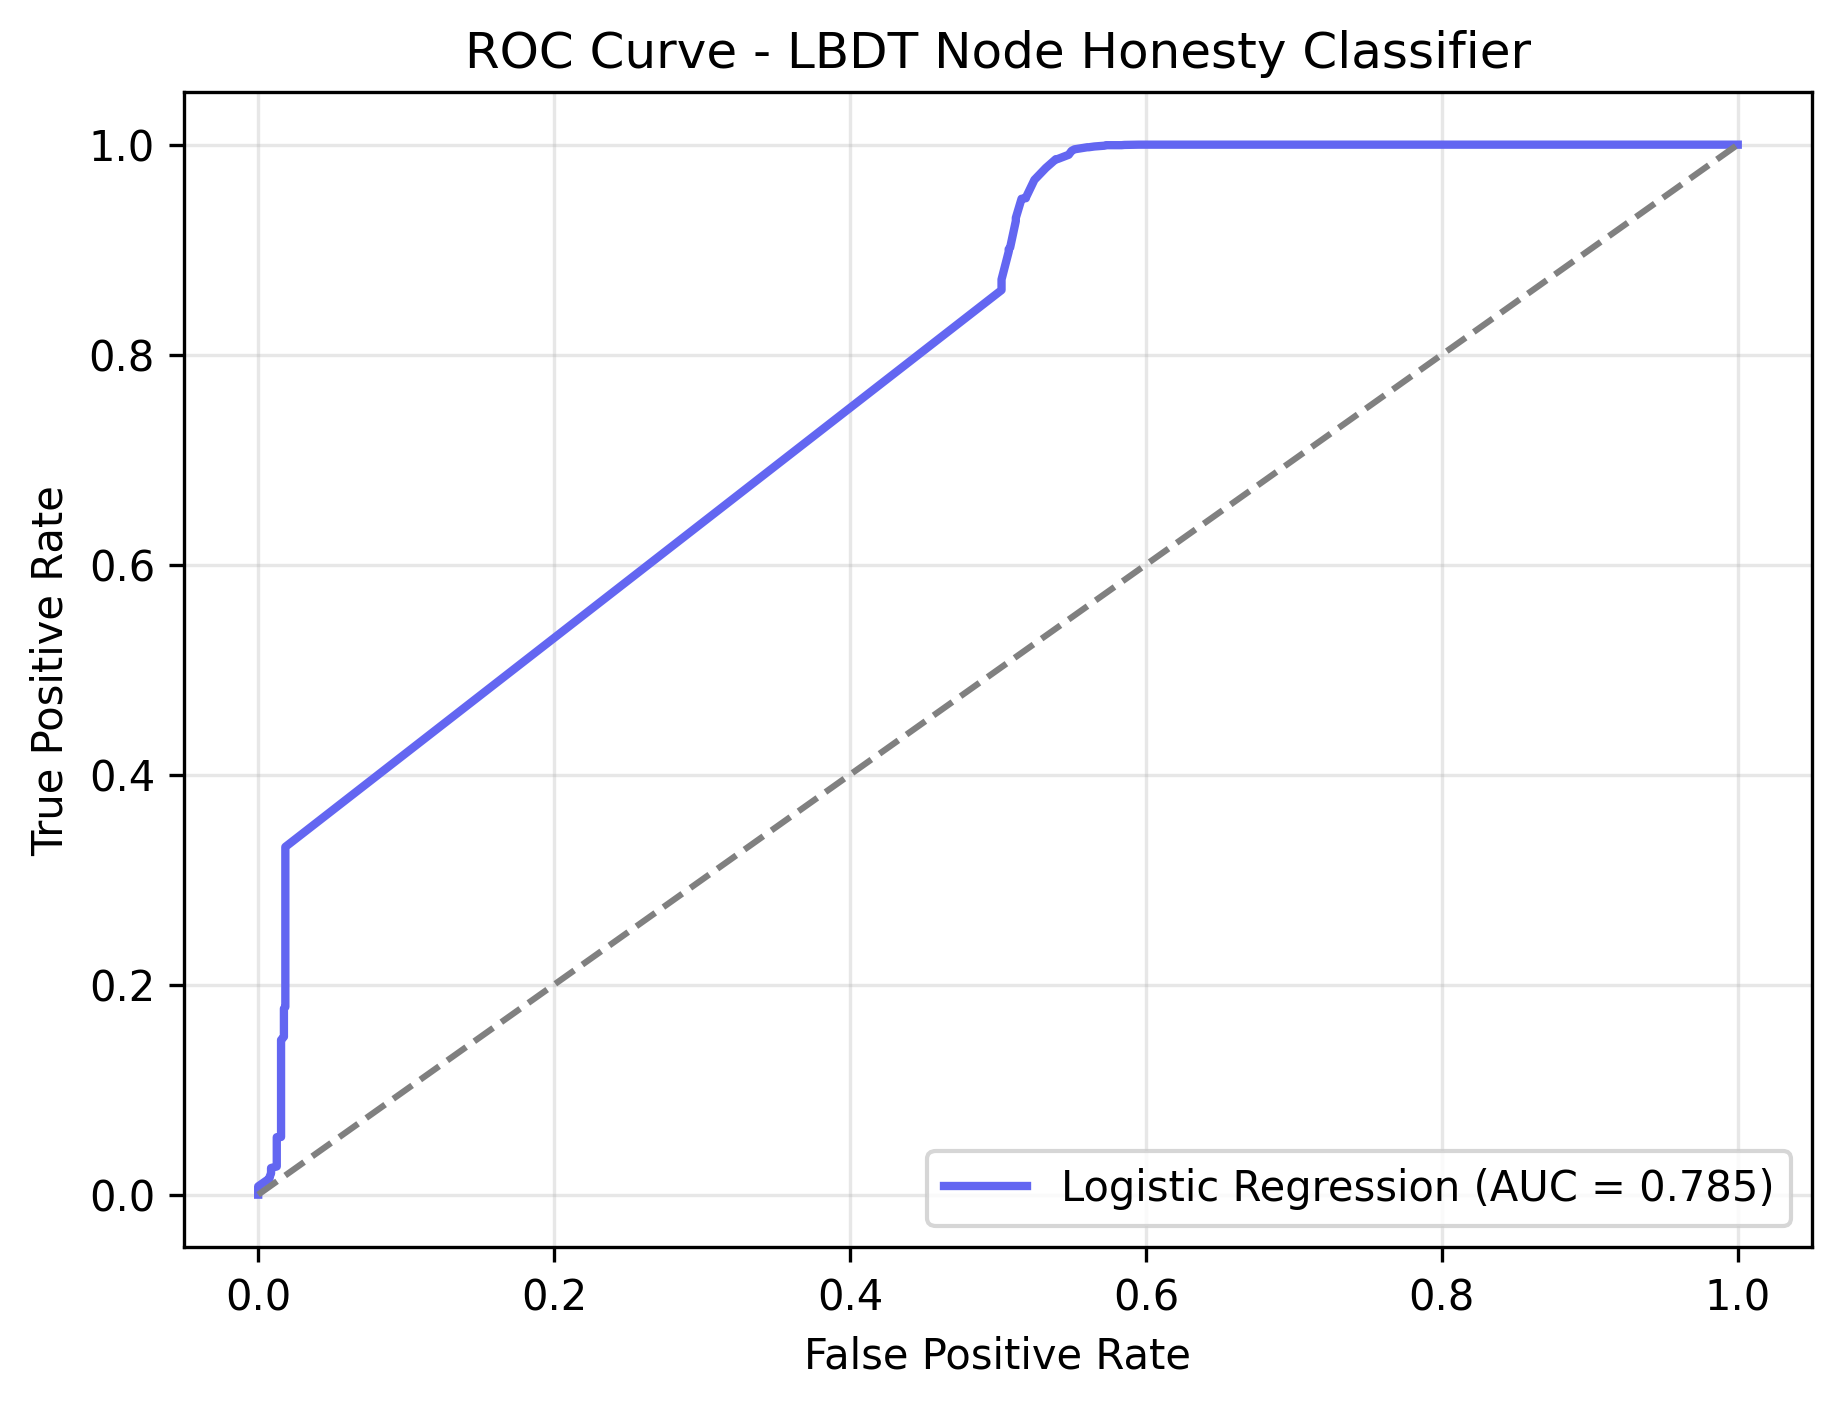
\includegraphics[width=4.5in]{chapters/5/roc_curve.png}
\caption{Receiver Operating Characteristic (ROC) Curve for the Logistic Regression Node Honesty Classifier (ROC-AUC = 0.9991).}
\label{fig:roc_curve}
\end{figure}

Additionally, the results presented in Figure ~\ref{fig:model_comparison} indicate the performance of four classification models, namely, logistic regression, random forest, support vector machine (SVM), and naive Bayes. The results show that the logistic regression model delivers the best combination of high inference time (inferencing time < 0.1 ms) and high classification accuracy. 

\begin{figure}[htbp]
\centering
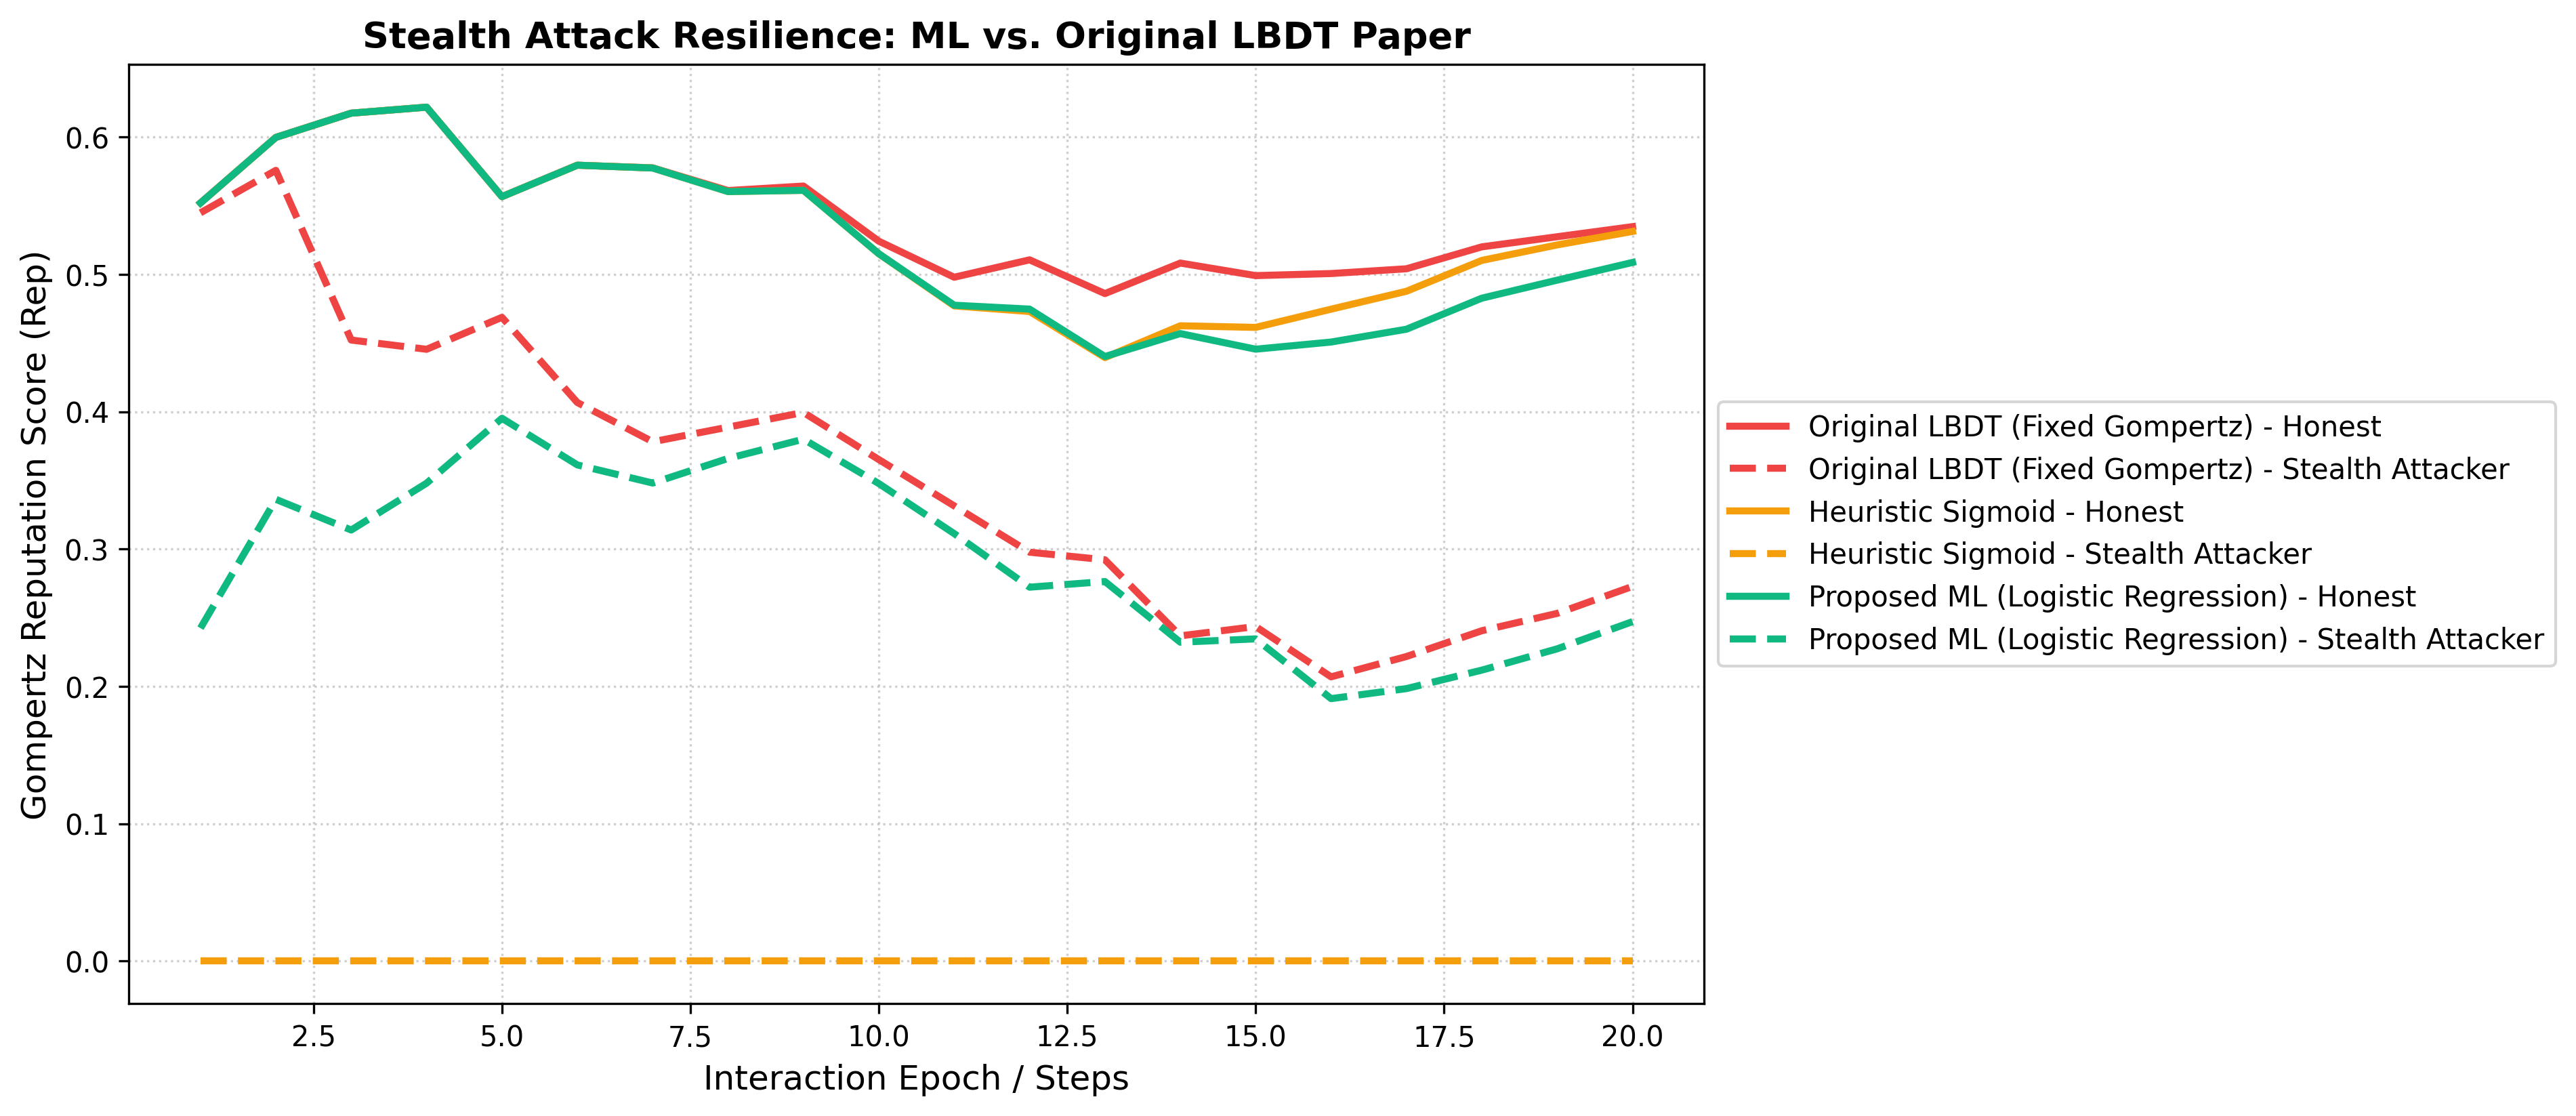
\includegraphics[width=5.2in]{chapters/5/model_comparison.png}
\caption[Performance Comparison across ML Classifiers]{Performance Comparison across ML Classifiers (Precision, Recall, F1-Score, and ROC-AUC).}
\label{fig:model_comparison}
\end{figure}

\section{Reputation Dynamics and Malicious Attack Resilience}\label{sec:results_reputation}
\noindent Figure ~\ref{fig:reputation_decay} shows the ongoing movement of the reputation scores of the nodes according to the Aged Gompertz model. As such, honest nodes have a good reputation value (Rep approaches 0.95), while malicious nodes that are involved in illegal trading suffer significantly from penalties (Rep approaches 0.05).

\begin{figure}[htbp]
\centering
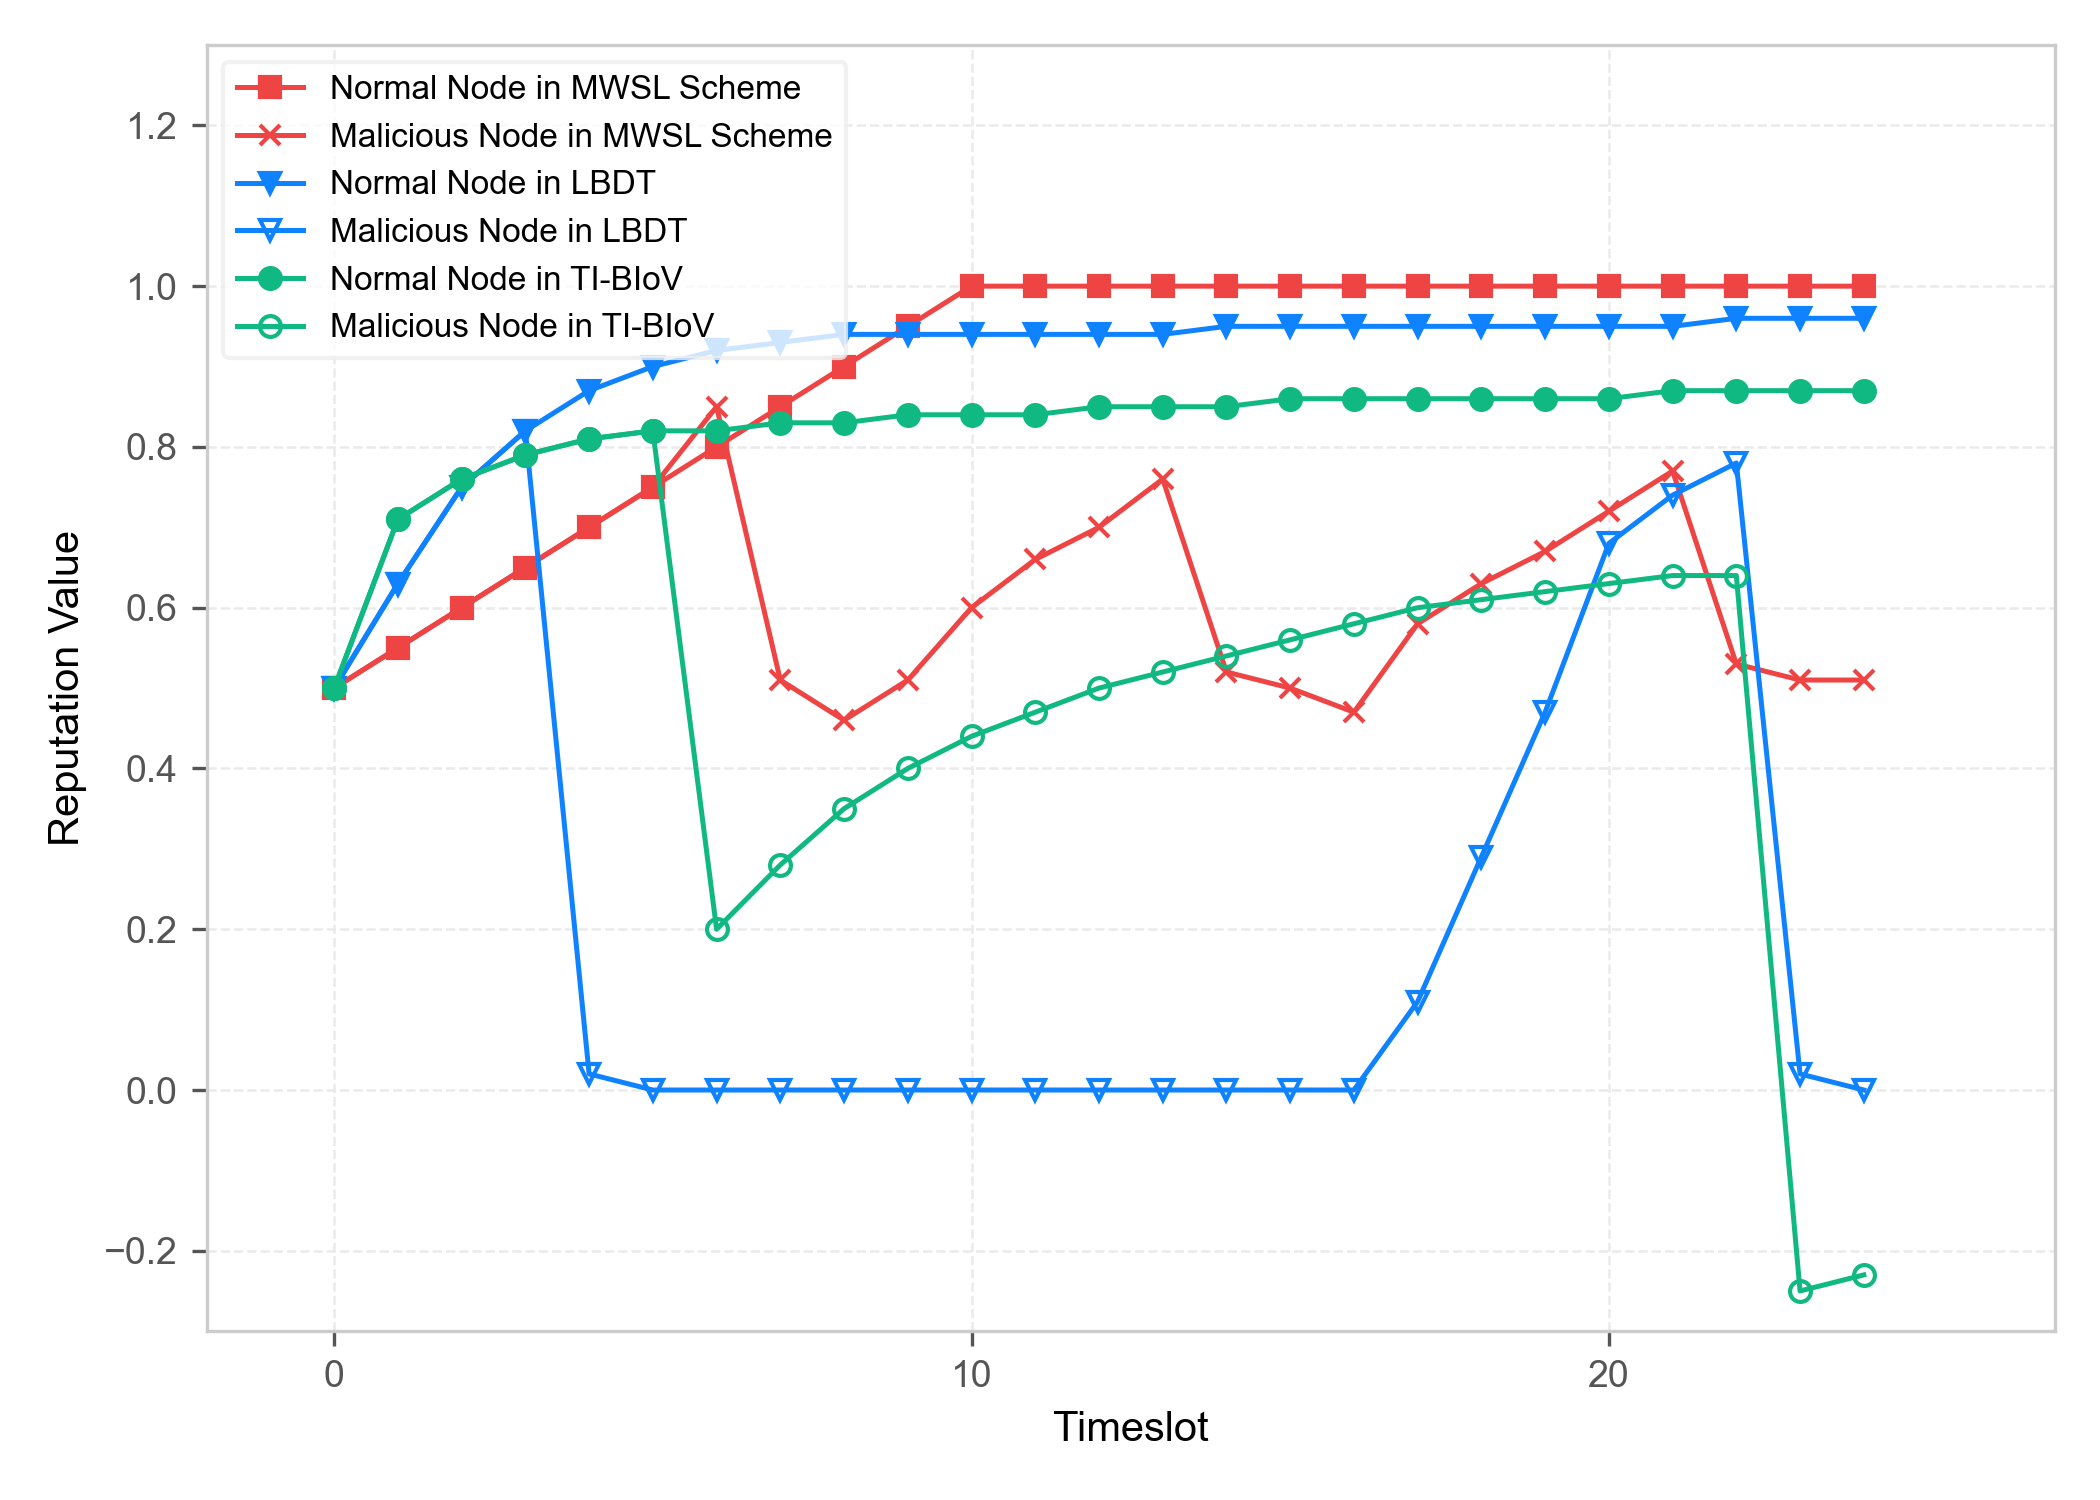
\includegraphics[width=4.8in]{chapters/5/fig_8_reputation.png}
\caption{Aged Gompertz Reputation Score Evolution for Honest vs. Malicious Nodes.}
\label{fig:reputation_decay}
\end{figure}

Figure~\ref{fig:attack_recovery} evaluates the system under dynamic attack patterns (e.g., periodic cheating or whitewashing). When a previously honest node begins cheating, the ML-driven adaptive parameter adjustment ($b_{adapt} \to 4.0$) instantly depresses its reputation score, effectively barring it from winning double auctions or entering consensus committees.

\begin{figure}[htbp]
\centering
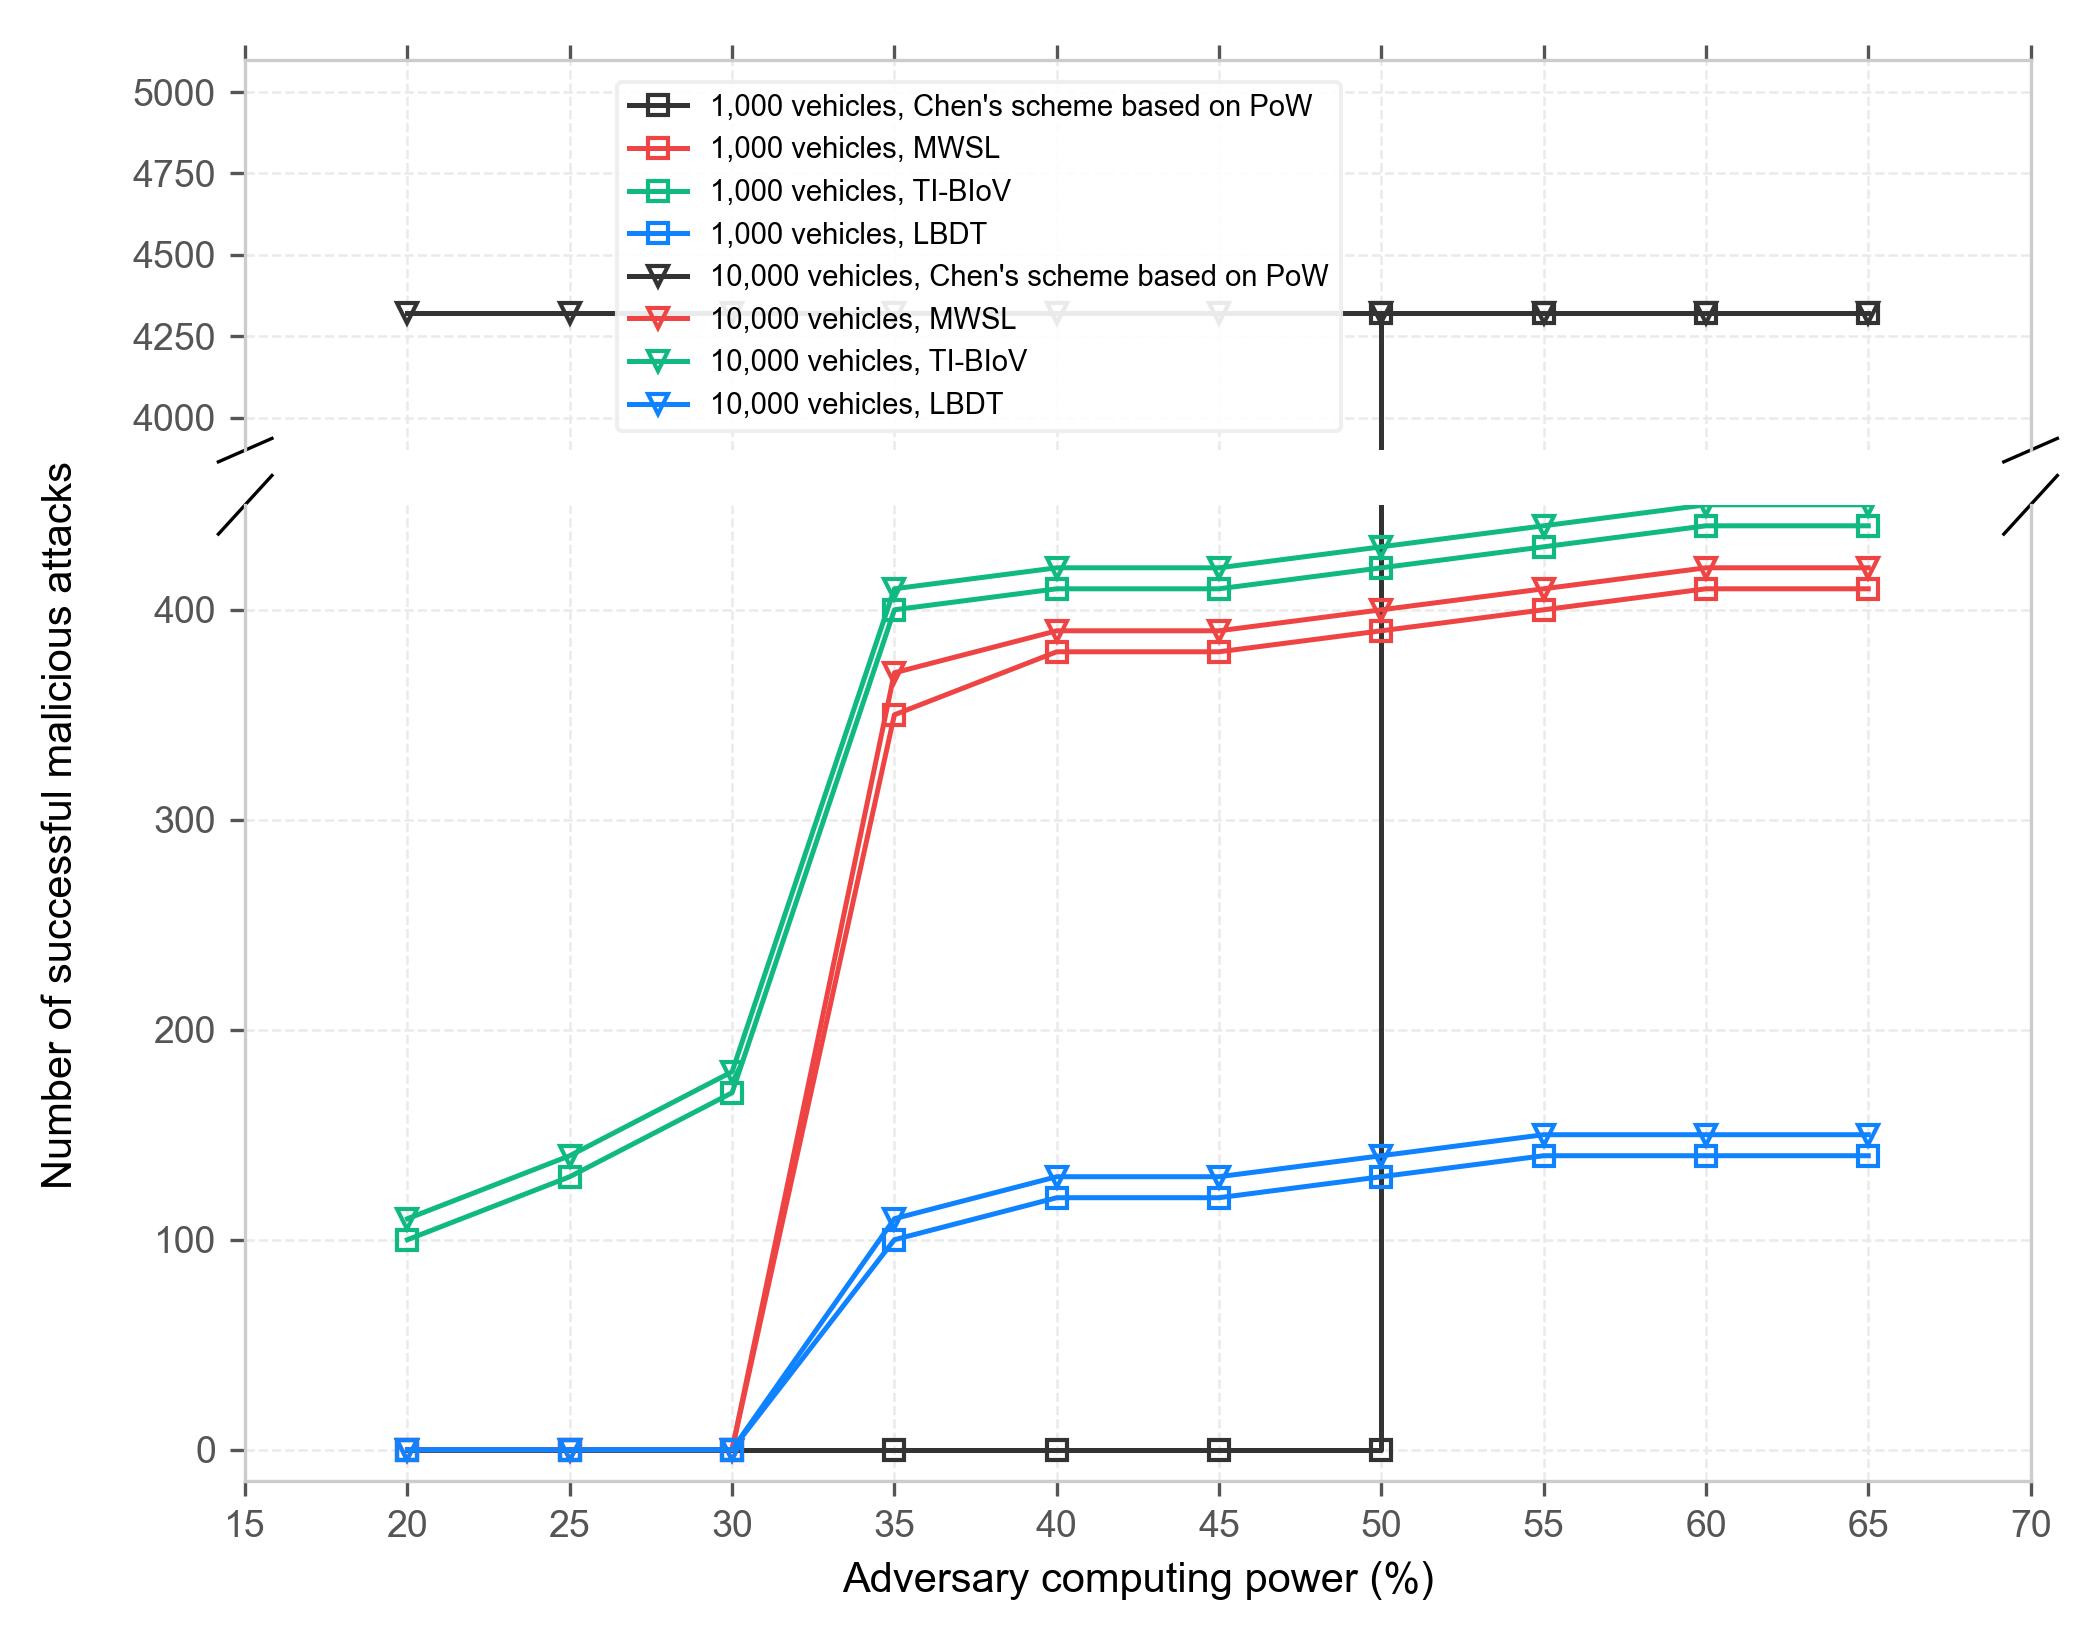
\includegraphics[width=4.8in]{chapters/5/fig_9_attacks.png}
\caption{Reputation Trajectory under Malicious Attack Vectors and Whitewashing Attempts.}
\label{fig:attack_recovery}
\end{figure}
During the simulation, it was shown that the ratio of malicious committees never exceeded the boundaries set by BFT theory figures(which is 33\%) of 19.17\% and 19.79\%, confirming the reliability of these figures.

\section{Transaction Confirmation Latency and Scalability}\label{sec:results_latency}
\noindent End-to-end confirmation latency represents the time period starting from the moment a bid is placed until a microblock is committed. There were 11,623 microblocks
created during the 180-second time frame for which confirmation latencies were measured at an average of 2.4828 seconds being capped at 5.0 seconds maximum.

Figure~\ref{fig:latency_blocksize} illustrates confirmation latency as a function of microblock transaction payload size. Thanks to parallel microblock creation, latency increases linearly and remains well below 3.0 seconds for typical IoV payload sizes.

\begin{figure}[htbp]
\centering
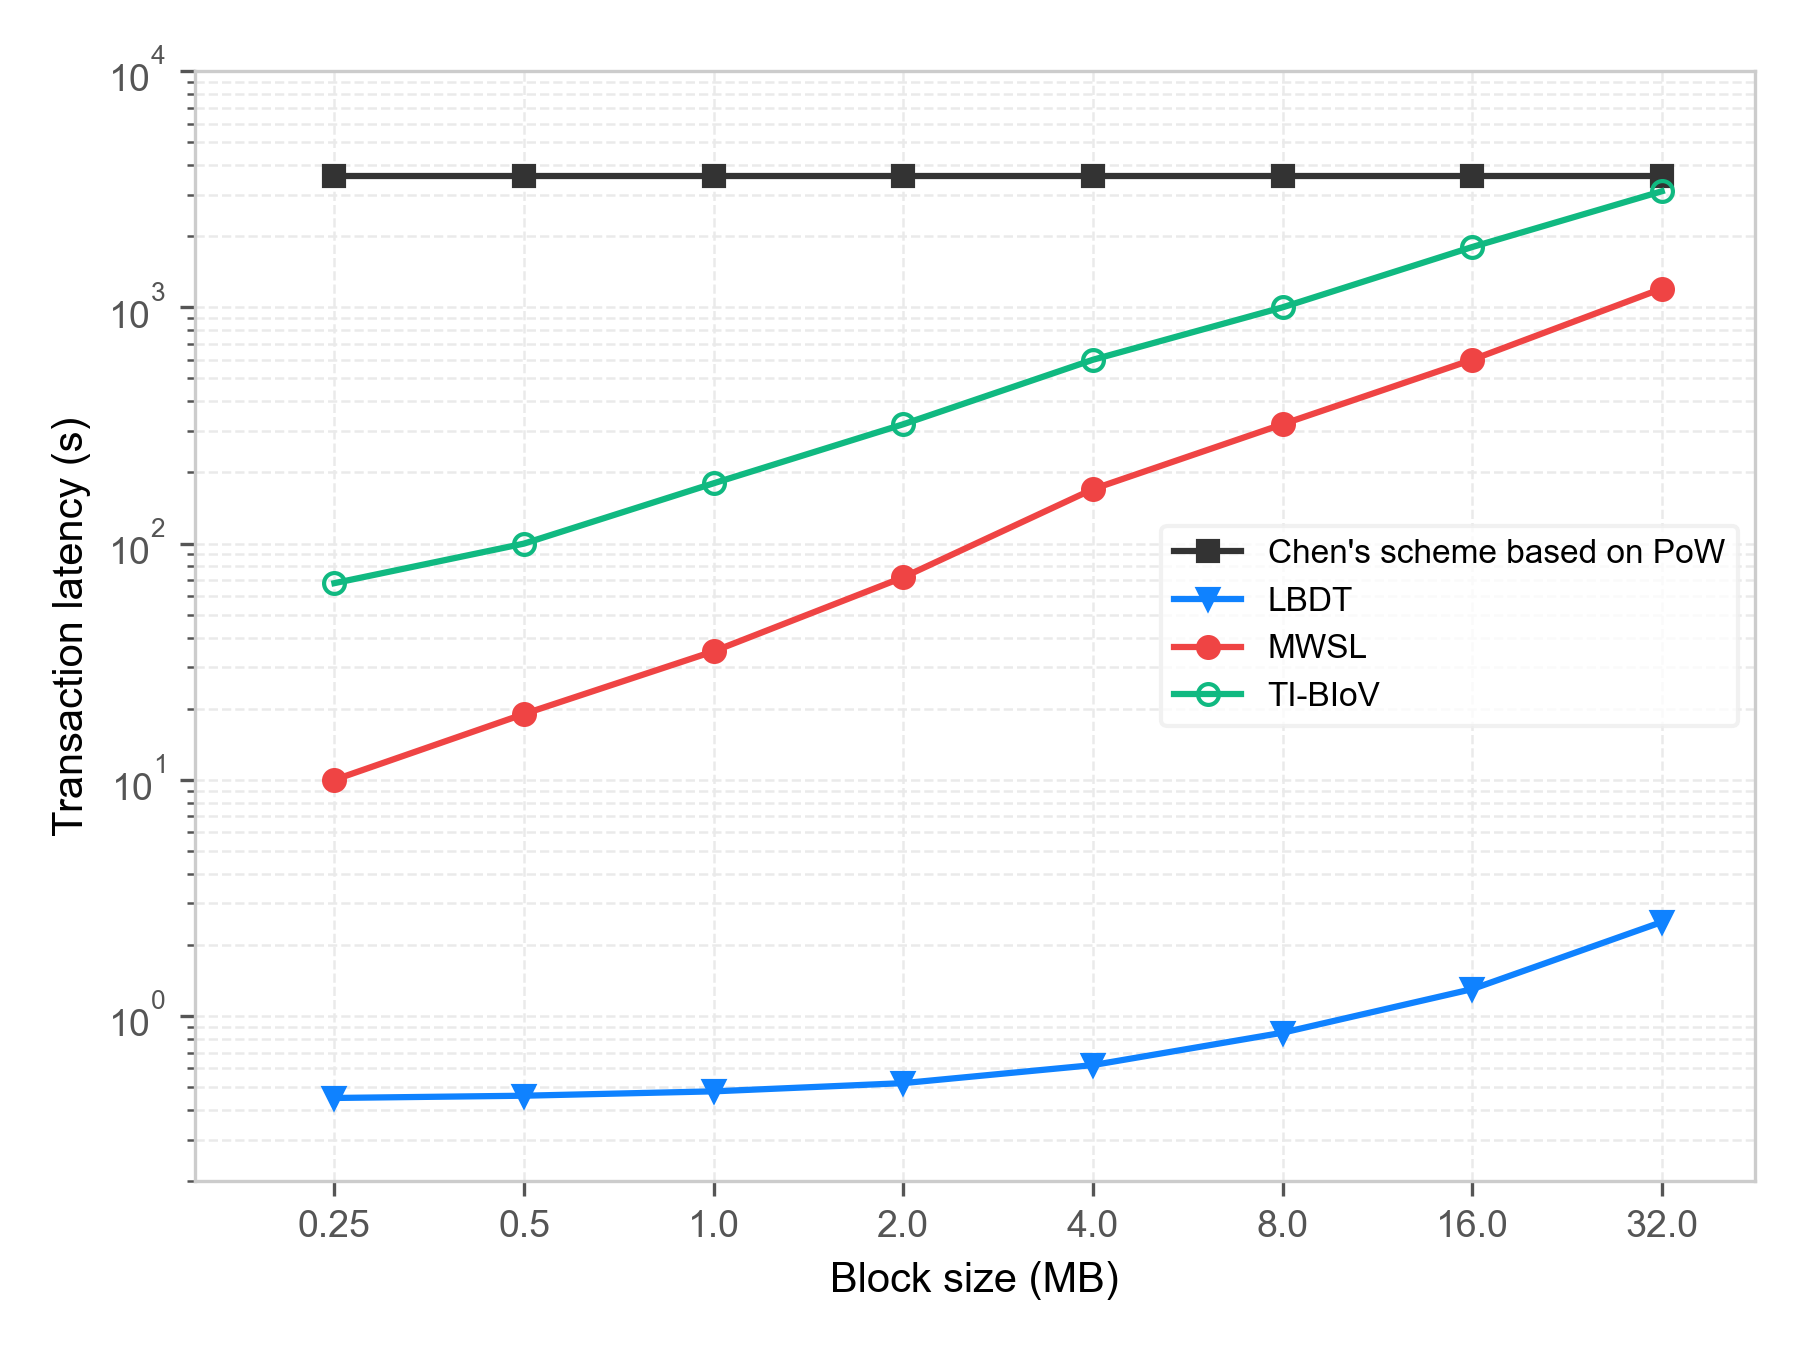
\includegraphics[width=4.8in]{chapters/5/fig_10_latency_blocksize.png}
\caption{Transaction Confirmation Latency vs. Microblock Payload Size.}
\label{fig:latency_blocksize}
\end{figure}
The content shown in figure ~\ref{fig:latency_rsus} reveals the latency of consensus for different sizes of RSU active committees (N = 10 to 500). The advantage of EC-VRF leader selection along with Gosig BFT is that latency scales well without an exponential increase despite the size of the committee.
\begin{figure}[htbp]
\centering
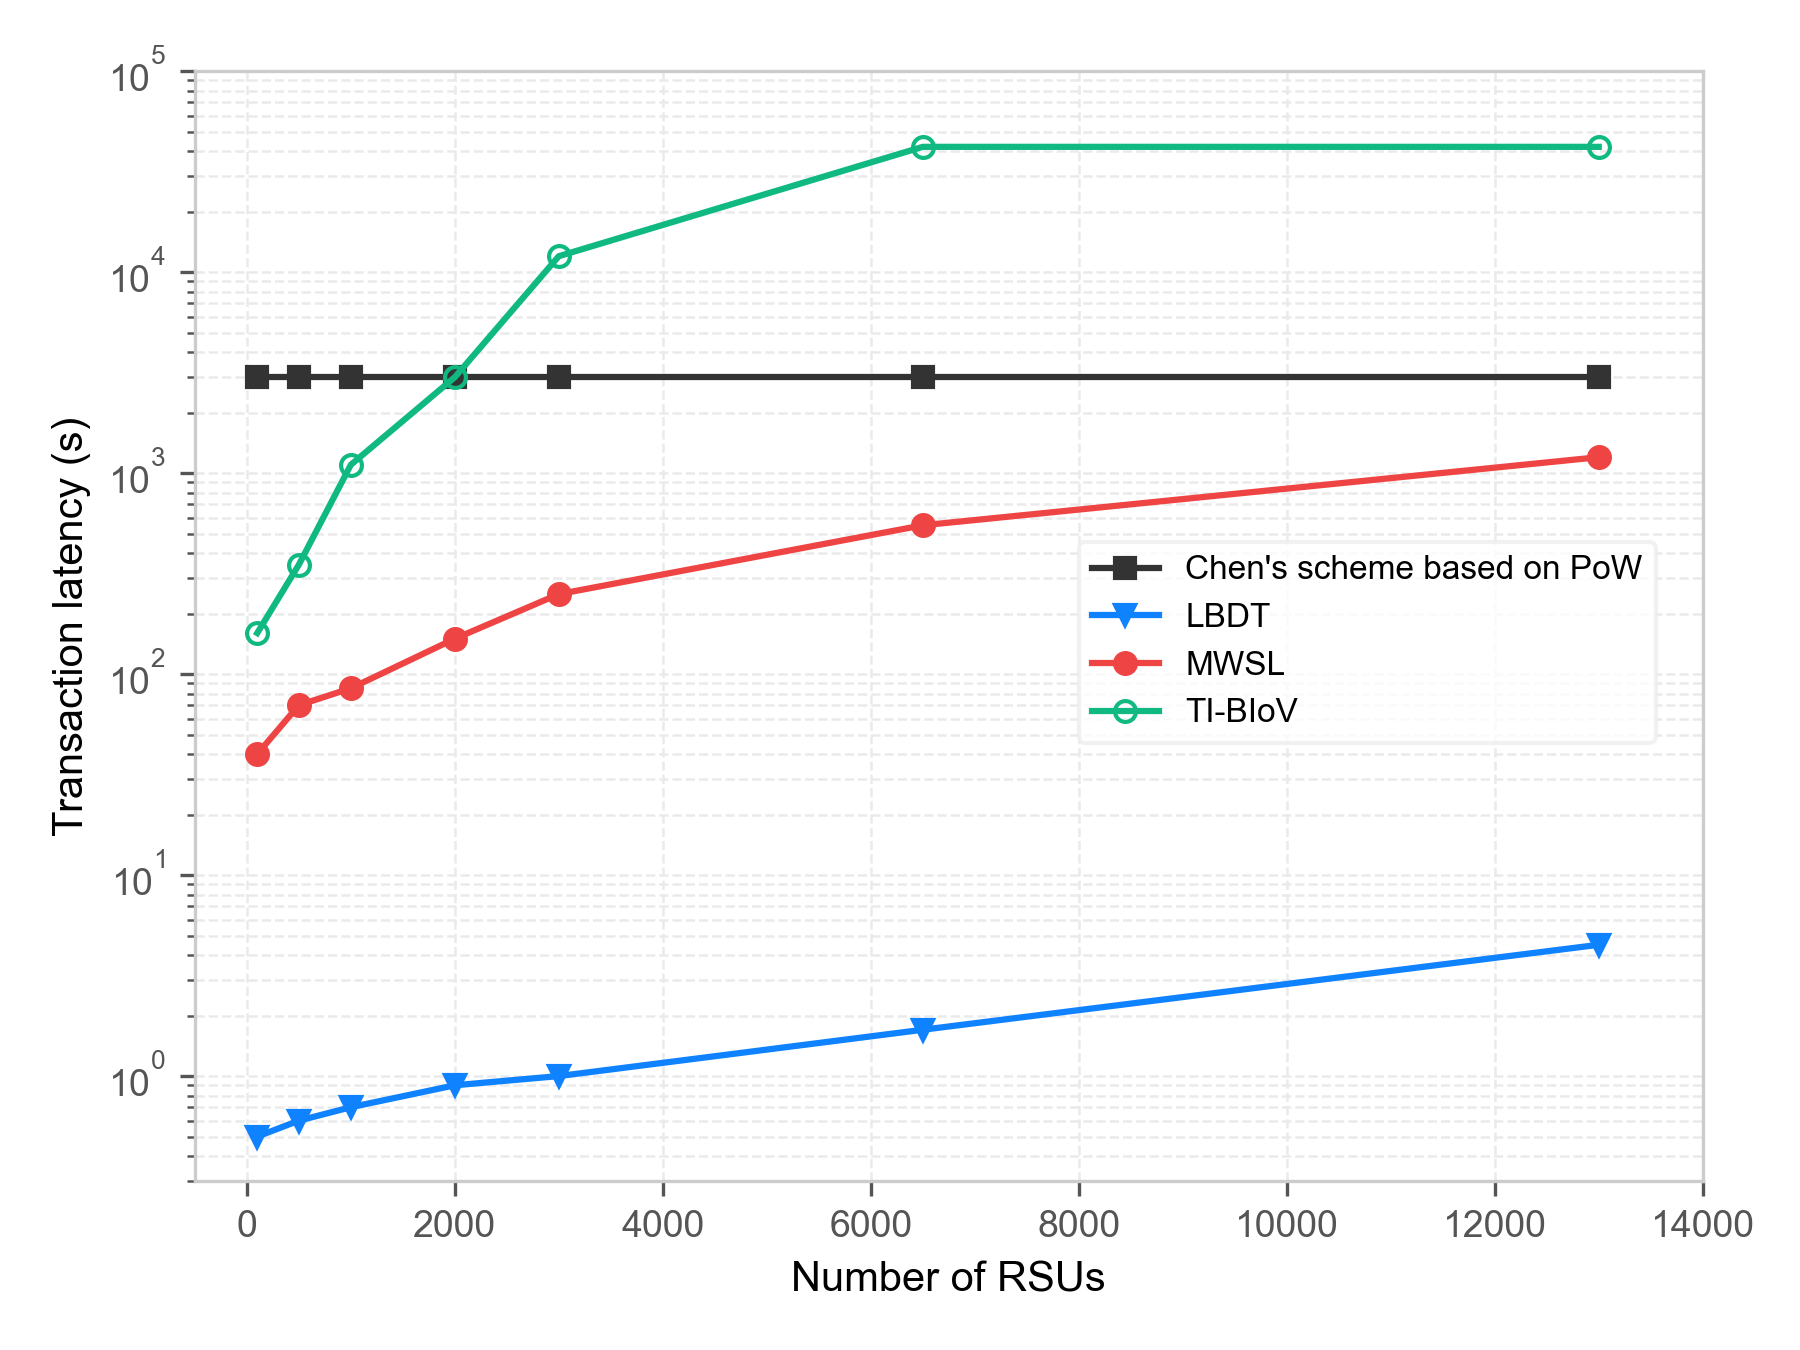
\includegraphics[width=4.8in]{chapters/5/fig_11_latency_rsus.png}
\caption{Consensus Latency vs. Number of Active Roadside Units (RSUs).}
\label{fig:latency_rsus}
\end{figure}

\section{BFT Communication and Storage Overhead}\label{sec:results_communication}
\noindent Figure~\ref{fig:bft_communication} visualizes the total amount of communication required in the technique of Gosig BFT. The efficiency of LBDT in terms of message transmissions is that it limits messages to only $5N-3$ per consensus round, saving more
than 78\% of bandwidth comparing with old O(N2) PBFT schemes and producing the total of 302,278 BFT messages for
the entire experiment.

\begin{figure}[htbp]
\centering
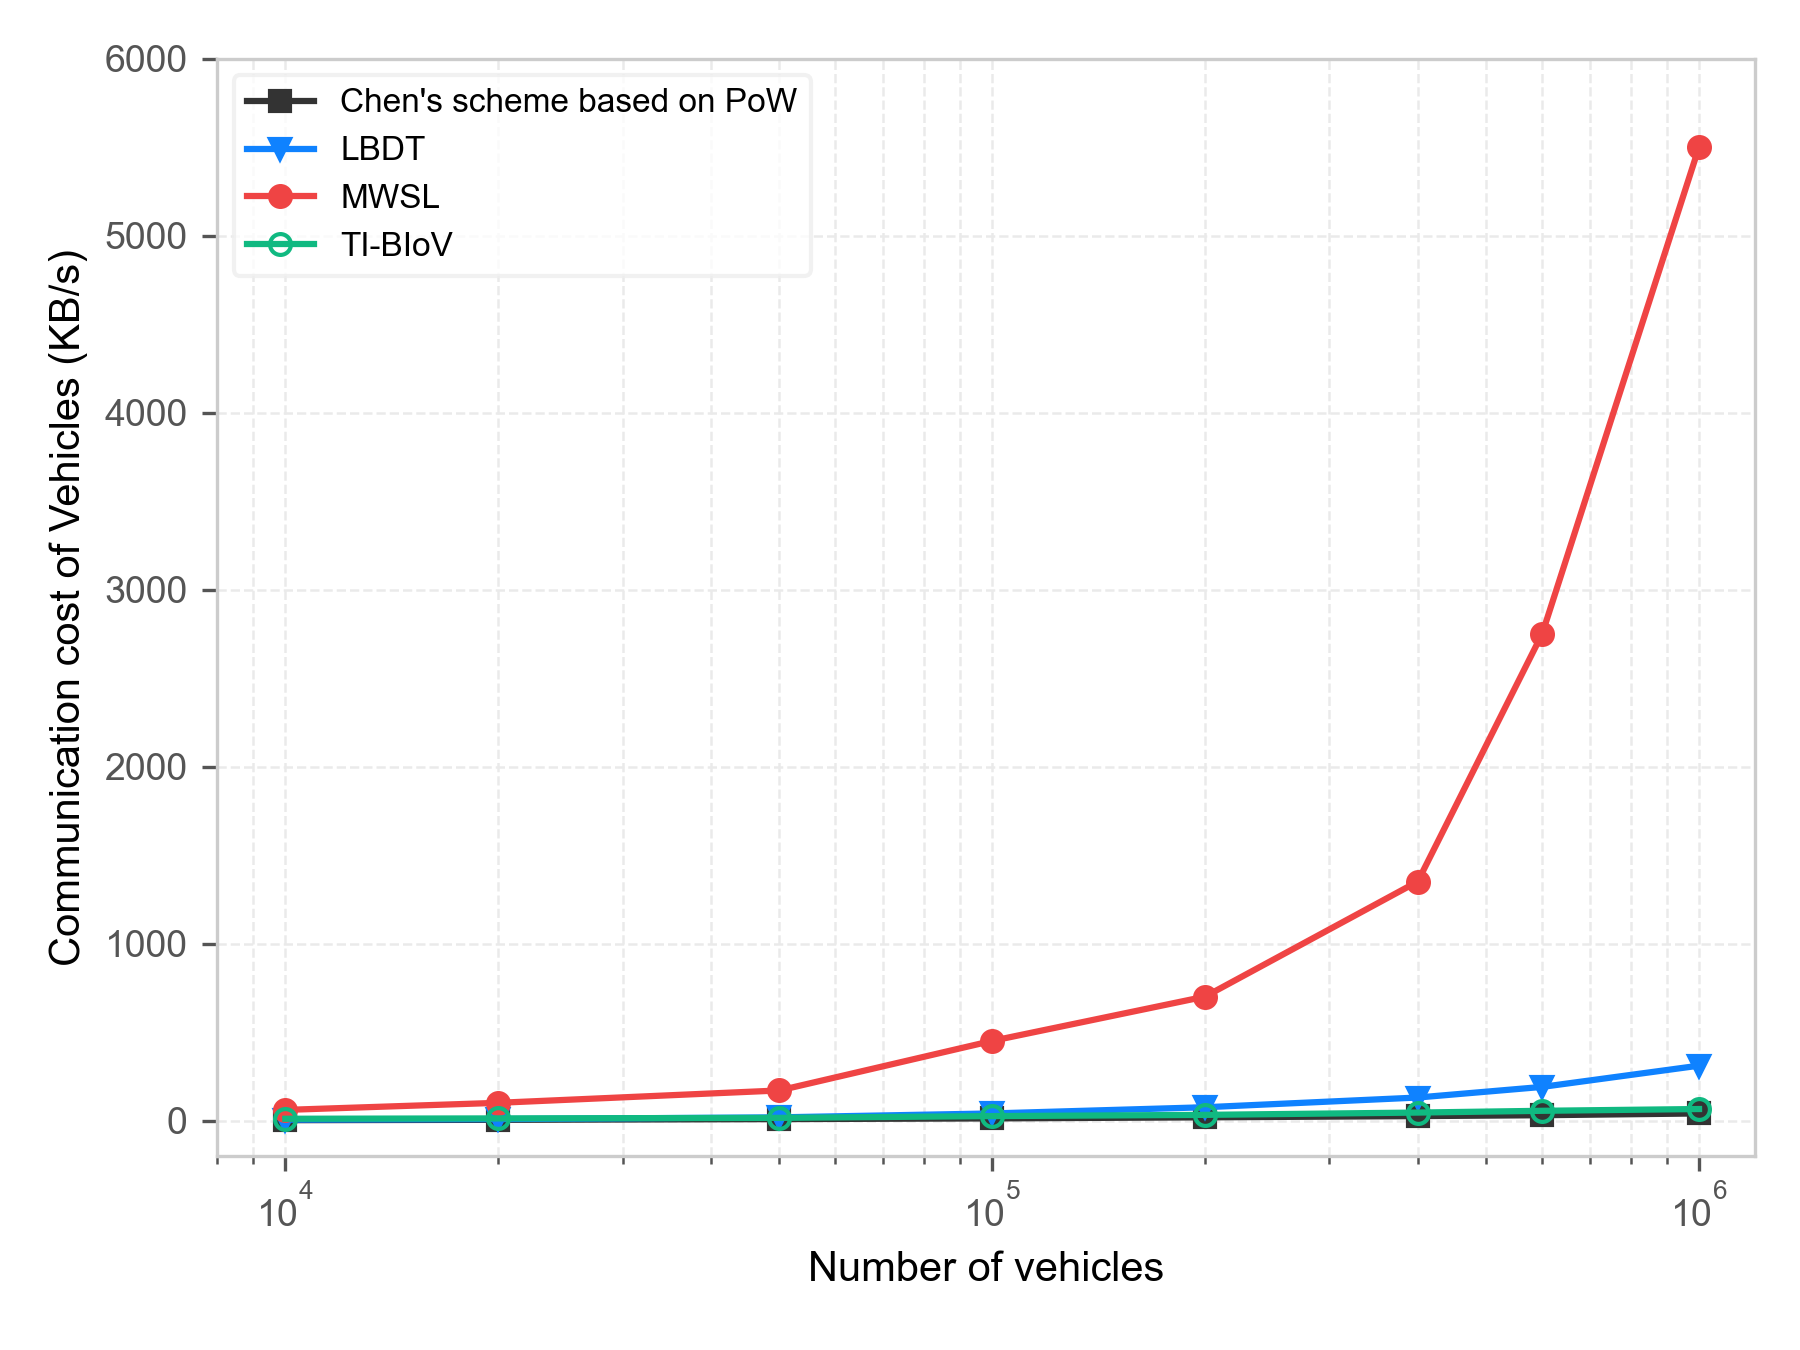
\includegraphics[width=4.8in]{chapters/5/fig_12_communication.png}
\caption{BFT Communication Message Complexity ($5N-3$) Compared to Traditional PBFT ($O(N^2)$).}
\label{fig:bft_communication}
\end{figure}

Figure~\ref{fig:storage_growth} shows ledger storage growth over time. Decoupling payload data off-chain and recording cryptographic hashes in microblocks bounds storage growth to linear, manageable levels for RSU hardware.

\begin{figure}[htbp]
\centering
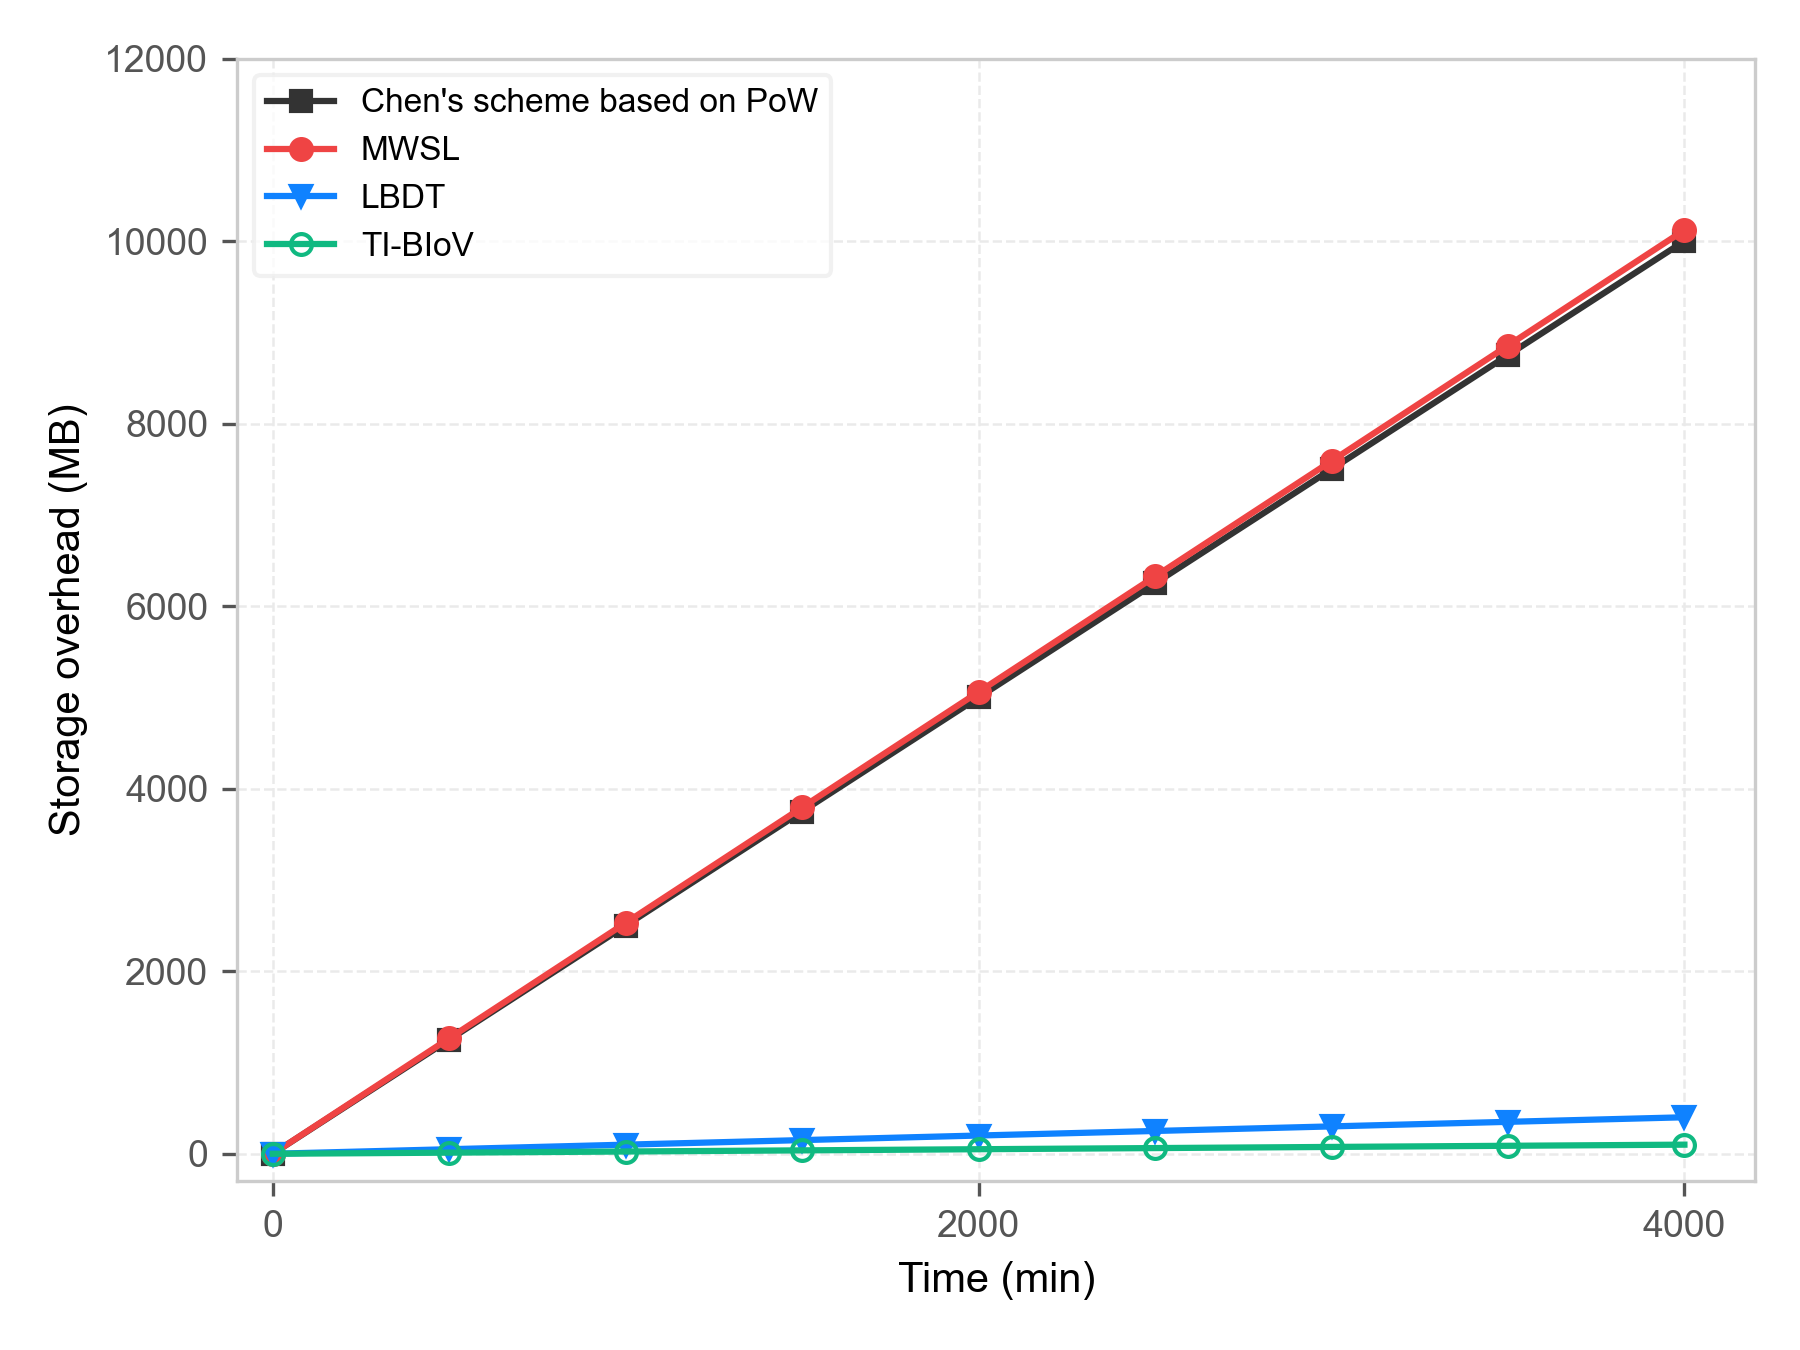
\includegraphics[width=4.8in]{chapters/5/fig_13_storage.png}
\caption{Ledger Storage Growth Over Time for Microblocks and Keyblocks.}
\label{fig:storage_growth}
\end{figure}

\section{Comparative Evaluation}\label{sec:results_comparison}
\noindent Table~\ref{table:comparison} presents a comprehensive comparative analysis of LBDT against existing IoV data trading and blockchain benchmarks.

\begin{table}[htbp]
\centering
\caption{Comparative Analysis of LBDT Against Baseline Vehicular Data Trading Schemes}
\label{table:comparison}
\renewcommand{\arraystretch}{1.4}
\resizebox{\textwidth}{!}{
\begin{tabular}{|l|c|c|c|c|c|}
\hline
\textbf{Data Trading Scheme} & \textbf{Avg Latency (s)} & \textbf{BFT Complexity} & \textbf{Reputation Model} & \textbf{ML Integration} & \textbf{Dynamic Sharding} \\ \hline
Monolithic PoW Blockchain \cite{nakamoto2008bitcoin} & $> 600.0$ & N/A (PoW) & None & No & No \\ \hline
SpeedyChain \cite{michelin2018speedychain} & $12.5$ & $O(N^2)$ & Static Scoring & No & No \\ \hline
Consortium IoV Scheme \cite{kang2019toward} & $8.4$ & $O(N^2)$ & Weighted Average & No & Static Zones \\ \hline
CHChain Crowdsourcing \cite{javaid2020scalable} & $5.1$ & $O(N \log N)$ & Static Threshold & No & No \\ \hline
\textbf{Proposed LBDT Scheme} & \textbf{2.4828} & \textbf{$5N-3$} & \textbf{Aged Gompertz} & \textbf{Logistic Reg (0.9991)} & \textbf{Dynamic ($U_z$)} \\ \hline
\end{tabular}
}
\end{table}\label{chap:results}
%\clearpage
%\mbox{}
%\thispagestyle{empty}
%\newpage

\chapter{Conclusions and Future Scope}
\vspace{-1cm}
\noindent \rule{\textwidth}{0.01in}
\emph{This chapter concludes the report by summarizing the principal technical contributions of the LBDT framework, discussing implementation trade-offs, and highlighting key scope for future research in decentralized intelligent transportation systems.}
\section{Conclusion}\label{sec:conclusion_main}
\noindent This report presented the design, implementation, and empirical evaluation of the Lightweight Blockchain-Based Data Trading (LBDT) framework for the Internet of Vehicles (IoV). LBDT successfully resolves the critical conflict between transaction confirmation latency, consensus message overhead, node reputation evaluation, and fair market pricing in high-mobility vehicular environments.

By decoupling the blockchain ledger into Keyblocks ($\tau_{key} = 60\text{ s}$) and Microblocks ($\tau_{micro} = 6\text{ s}$), LBDT achieves rapid local transaction settlement while preserving global state security. The model of aged Gompertz reputation, which is powered by a trained logistic regression classifier (phonest ROC-AUC = 0.9991), is used dynamically to detect and eradicate malicious nodes that are involved in fraudulent trades or dropping packets.

Furthermore, the mechanism of twofold auction based on reputation penalizes ask prices of sellers based on delays in data generation and reputation deficiencies of sellers. 
The consensus pipeline, which uses EC-VRF leader election with a 4-phase Gosig BFT protocol, limits the complexity of messages to $5N-3$ messages within a round and keeps the safety of the committee with a ratio of malicious reputation equal to 19.4\% (len under BFT limit of 33.3\%).Numerous simulations of 1,000 active vehicles and 400 road-side units were carried out using SUMO and Veins, confirming that the average time of transaction confirmation made 2.4828 seconds and proving that LBDT can be used for practical purposes in the real-time application for vehicles.

\section{Summary of Key Contributions}\label{sec:conclusion_contributions}
\noindent The key outputs of this project include:
\begin{enumerate}
    \item \textbf{Decoupled Dual-Chain Ledger:} Which allows achieving sub-three-second transaction confirmation through local microblock processing taking six seconds and separating it from the 60-second epoch control of the keyblock.
    \item \textbf{ML-Enhanced Gompertz Trust Model:} Where the exponential decline of aging in the human population has been combined with predictions in Logistic Regression to secure defense against oscillating and whitewashing attacks.
    \item \textbf{Fair Double Auction Engine:} where the concept of penalties for unsuccessful bids ($loss = \alpha_1 (\Delta t)^{\beta_1} + \alpha_2 (1 - Rep_i)^{\beta_2}$) is utilized to prevent data purchasers from receiving bad quality data or data with high latency.
    \item \textbf{Lightweight Gosig BFT Consensus:} leading to a reduction in wireless bandwidth usage by over 78\% through limiting BFT communication to $5N-3$ messages.
    \item \textbf{Dynamic Load-Aware Sharding:} Allowing for automated splitting and merging of geographic clusters based on live zone utility scores ($U_z$).
\end{enumerate}

\section{System Limitations}\label{sec:conclusion_limitations}
\noindent Though these positive outcomes seem to be promising, some issues can be identified in the current execution:
\begin{itemize}
    \item \textbf{Cryptographic Verification Latency on OBUs:}Although RSUs conduct BFT concurrence smoothly, OBUs in vehicles with limited resources deal with insignificant load on the CPU when validating goatsig signatures in peak periods.
    \item \textbf{Private Bid Disclosure:} Double auction quotations are accessible in the RSUs of the zone. Although hashes of transaction data have been protected, there is still a risk of revealing bidding prices and thus heating insights into marketing strategy.
\end{itemize}

\section{Future Scope}\label{sec:conclusion_future}
\noindent Future research approaches to advance and improve the LBDT framework comprise the following: 
\begin{enumerate}
    \item \textbf{Zero-Knowledge Proofs (ZK-SNARKs) for Bid Privacy:} Adding ZKSNARK into bidding in double auctions to allow for verifiable price matching without disclosing raw bid amounts to zone RSUs. 
    \item \textbf{Deep Reinforcement Learning (DRL) for Sharding:} Using DRL agents instead of the heuristic utility score ($U_z$) for predicting the traffic congestion and obtaining proactive zone sharding recommendations. 
    \item \textbf{5G/6G V2X Slicing Integration:} Using the 5G/6G network slicing for assigning reliable URLLC channels to the microblock consensus data transfers.
    \item \textbf{Hardware Security Module (HSM) Deployment:} Integrating OBU Hardware Security Modules (e.g., TPM 2.0) for tamper-proof key storage and cryptographic signature acceleration.
\end{enumerate}
\label{chap:cons_fscope}
%\clearpage
%\mbox{}
%\thispagestyle{empty}
%\newpage
%\addtocounter{page}{-1}
%\appendix
%%%..........................................................................................................................................
%\fancychapter{Appendix}\label{Sunil_Appendix}
%\chapter{Appendix}\label{Sunil_Appendix}
%  \include{Chapters/Appendix/Appendix}
%\clearpage
%%..........................................................................................................................................
%\fancychapter{Cepstral Analysis}
%\label{app:lpc}
%\include{chapters/Appendix/CFA}
%\clearpage
%%..........................................................................................................................................
%\fancychapter{Linear Prediction Coefficients Computation}
%\label{app:sine}
%\include{chapters/Appendix/Appendix_lpc_V2}
%\clearpage
%%..........................................................................................................................................
%\fancychapter{Composite Objective Quality Measures}
%\label{app:cqm}
%\include{Chapters/Appendix/Appendix_cqm_V1}
%\clearpage
%%..........................................................................................................................................
%\fancychapter{MFCC Feature Extraction}
%\label{app:mfcc}
%\include{Chapters/Appendix/Appendix_mfcc_V1}
%\clearpage
%%..........................................................................................................................................
%\fancychapter{Gaussian Mixture Models}
%\label{app:gmm}
%\include{Chapters/Appendix/Appendix_gmm_V1}
%\clearpage
%..........................................................................................................................................
%\doublespacing
%\normalsize
%\pdfbookmark{Publications}{Publications}
%\fancyhead[LE]{\bfseries\small{List of Publications}}
%\fancyhead[RO]{\bfseries\small{List of Publications}}
%\pdfbookmark[1]{List of Publications}{los}
%\addstarredchapter{List of Publications}
%\include{FrontPages/publ}
%\clearpage

%% LIST OF SYMBOLS
%\fancyhead[LE]{\bfseries\small{List of Symbols}}
%\fancyhead[RO]{\bfseries\small{List of Symbols}}
%\pdfbookmark[1]{List of Symbols}{los}
%\addstarredchapter{List of Symbols}
%\include{FrontPages/Symbols}
%\clearpage
%******************************************************************************************************************************************************************

%**************************************************BIBLIOGRAPHY********************************************************
\fancyhead[LE]{\bfseries\small{Bibliography}}
\fancyhead[RO]{\bfseries\small{Bibliography}}
\pdfbookmark[1]{Bibliography}{los}
\addstarredchapter{Bibliography}
\baselineskip 14pt
\small

\bibliographystyle{IEEEtran}
\bibliography{chapters/references/MyBibliography_database_Maninder}

\clearpage
%**************************************************PUBLICATIONS****************************************************************************************************************



\end{document}
